%\documentclass[letterpaper,twocolumn,fleqn]{sig-alternate-10pt}
\documentclass[10pt, sigconf, printonly]{acmart}

\settopmatter{printacmref=false, printccs=false, printfolios=false}
\setcopyright{rightsretained}
\renewcommand\footnotetextcopyrightpermission[1]{} % removes footnote with conference information in first column
\pagestyle{plain} % removes running headers

\paperheight 11in
\paperwidth 8.5in
\usepackage{geometry}
\usepackage{epsfig,endnotes}
\usepackage[export]{adjustbox}
\usepackage{tabularx}
\usepackage{appendix}
\newcommand{\sysname}{Tagger}

\usepackage{url}
%\usepackage{cite}
\usepackage{lineno}
\renewcommand\linenumberfont{\normalfont\bfseries\small}
\usepackage{pifont}
\usepackage{epsfig,epsf,url,amssymb}
\usepackage{tabularx}
\usepackage[ruled,vlined]{algorithm2e}
\usepackage{amsmath}
\usepackage{mathtools}
\newtheorem{mydef}{Definition}
\usepackage{rotating}
\usepackage{wrapfig}
\usepackage{times}
\long\def\comment#1{}
\usepackage{multirow}
\usepackage{lscape}
\usepackage{stmaryrd}
\usepackage{wrapfig}
\usepackage{hhline}
\usepackage{textcomp,booktabs}
\usepackage{color}
\usepackage{colortbl}
\usepackage{multirow}
\usepackage{rotating}
\usepackage{epstopdf}
\usepackage{url}
\usepackage{subfig}
\usepackage{graphicx}

\newcommand{\paraspace}{\vspace{0.05in}}
\newcommand{\para}[1]{\paraspace\noindent{\bf #1} }
\newcommand\fixme[1]{{\color{red} #1}}
\newcommand\yibo[1]{{\color{blue} #1}}
\newcommand\modified[1]{{\color{blue} #1}}

\def\naive{na\"\i ve}

\newcommand{\tabincell}[2]{\begin{tabular}{@{}#1@{}}#2\end{tabular}}

\newcommand{\subcaption}[1]{\centerline{#1}\vspace{0.1in}}
\long\def\comment#1{}
%\newtheorem{theorem}{Theorem}
%\newtheorem{lemma}[theorem]{Lemma}
%\newtheorem{proposition}[theorem]{Proposition}
%\newtheorem{corollary}[theorem]{Corollary}
%\newtheorem{problem}[theorem]{Problem}

%\def\BState{\State\hskip-\ALG@thistlm}
%
%\newenvironment{definition}[1][Definition]{\begin{trivlist}
%		\item[\hskip \labelsep {\bfseries #1}]}{\end{trivlist}}
%\newenvironment{problem}[1][]{\begin{trivlist}
%		\item[\hskip \labelsep {\bfseries}]}{\end{trivlist}}
%\newenvironment{remark}[1][Remark]{\begin{trivlist}
%		\item[\hskip \labelsep {\bfseries #1}]}{\end{trivlist}}
%% 
%% \newenvironment{icompact}{
%%   \begin{list}{$\bullet$}{
%%     \parsep 1pt plus 1pt
%%     \partopsep 1pt plus 1pt
%%     \topsep 1pt plus 2pt minus 1pt
%%     \itemsep 1.5pt plus 1pt
%%     \parskip 0pt plus 2pt
%%     \leftmargin 0.15in}
%%        }
%%   {\normalsize\end{list}}
%% 
%% \newenvironment{ecompact}{
%%   \begin{list}{$\bullet$}{
%%     \parsep 1pt plus 1pt
%%     \partopsep 1pt plus 1pt
%%     \topsep 1pt plus 2pt minus 1pt
%%     \itemsep 1.5pt plus 1pt
%%     \parskip 0pt plus 2pt
%%     \leftmargin 0.15in}
%%        }
%%   {\normalsize\end{list}}
%% 
%% 
\begin{document}
	\title{\sysname{}: Practical PFC Deadlock Prevention in\\Data Center Networks}
	\author{Shuihai Hu$^{1,2}$~~~Yibo Zhu$^{1}$~~~Peng Cheng$^{1}$~~~Chuanxiong Guo$^{1}$~~~\\Kun Tan$^{1}$~~~Jitendra Padhye$^{1}$~~~Kai Chen$^{2}$\\ 
		$^{1}$Microsoft ~~~$^{2}$Hong Kong University of Science and Technology}

\begin{abstract} Remote Direct Memory Access over Converged Ethernet (RoCE) deployments
		are vulnerable to deadlocks induced by Priority Flow Control (PFC).
		Prior solutions for deadlock prevention either require significant
		changes to routing protocols, or require excessive buffers in the
		switches. In this paper, we propose a scheme for deadlock prevention,
		called \sysname{}. It does not require any changes to the routing
		protocol, and needs only modest buffers.  \sysname{} is based on the
		insight that given a set of expected lossless routes, a simple tagging
		scheme can be developed to ensure that no deadlock will occur under any
		failure conditions. We design such a scheme, prove that it prevents
		deadlock and implement it efficiently on commodity hardware.
\end{abstract}

	\maketitle
	
	
	%\vspace{-0.1in}
\section{Introduction}
\label{sec:intro}

Public cloud providers like Microsoft and Google are deploying Remote Direct
Memory Access (RDMA) over Ethernet (RoCE) in their data centers to enable low
latency, high throughput data transfers with minimal CPU
overhead~\cite{dcqcn,timely}. Systems like Pilaf~\cite{pilaf}, Farm~\cite{farm},
TesnorFlow~\cite{tensorflow}, and CNTK~\cite{cntk} rely on RDMA/RoCE for
enhanced performance. 

RoCE uses Priority Flow Control (PFC) to prevent packet drops due to buffer
overflow at the switches. PFC allows a switch to temporarily pause its upstream
neighbor. While PFC is effective, it can lead to
deadlocks~\cite{rdmaatscale,tcpbolt,hu2016deadlocks}. Deadlocks are caused by
circular buffer dependency (CBD)~\cite{hu2016deadlocks}, {\em i.e.,} the occupied 
buffers are waiting for each other in a loop.

While CBD can be caused by a routing loop, routing loop is not required -- flows
that travel on loop-free paths can create buffer dependencies that lead to CBD.
A simple but contrived example is shown in Figure~\ref{fig:basic_deadlock}. We
will discuss more realistic scenarios (e.g. Figure~\ref{fig:clos_1_bounce})
later.  See~\cite{hu2016deadlocks} for several other examples. 

The deadlock problem is not merely theoretical -- our conversations with
engineers at large cloud providers confirm that they have seen the problem in
practice and at least one provider has reported it publicly~\cite{rdmaatscale}.
Deadlock is a serious problem because a deadlock is not transient -- once a
deadlock forms, it does not go away even after the conditions (e.g. a temporary
routing loop due to link failure) that caused its formation have
abated~\cite{rdmaatscale}. Worse, a small initial deadlock may cause the PFC
frames to propagate and create a global deadlock, and shutdown the whole
network.

Current solutions to the deadlock problem fall in two categories. The first
category consists of solutions that {\em detect} the formation of the deadlock
and then use various techniques to {\em break} it~\cite{shpiner2016unlocking}.
These solutions do not address the root cause of the problem, and hence cannot
guarantee that the deadlock would not immediately reappear.

The second category of solutions are designed to {\em prevent} deadlocks.  For
deadlock formation, CBD is {\em necessary}, but not {\em
sufficient}~\cite{hu2016deadlocks}. Unfortunately, {\em sufficient} conditions
for deadlock formation are not well understood~\cite{hu2016deadlocks}. Thus,
currently, preventing CBD is the only practical way to prevent deadlocks.

In \S\ref{sec:challenges}, using data from a large cloud provider's data
centers, we show that any practical deadlock prevention scheme must meet three
key challenges. These include: $(i)$ it should require no changes to existing
routing protocols or switch hardware, $(ii)$ it must deal with link failures and
associated  route changes, and $(iii)$ it must work with limited buffer
available in commodity switches.

Prior proposals for deadlock prevention fail to meet one or more of these
challenges.  Some schemes~\cite{infiniband,blazewicz1994optimal} require
centralized routing.  These are difficult to deploy in existing data centers.
Others are distributed, but brand-new routing
protocols~\cite{dally,duato93,dally93,sancho2004,flich2012survey,lash,wu2003fault,glass,duato2001,domke2011,puente1999,dfedst16,tcpbolt,dfedst16}
that are not supported by commodity switches.  Many of these schemes also
require carefully controlling the paths -- something that is simply not possible
with decentralized routing in presence of link failures~\cite{netpilot}.
Finally, some schemes~\cite{firstpaper,survey,datanetworks,karol2003prevention},
require creation of numerous priorities and buffer management according to those
priorities.  However, modern data center networks, built using commodity
switches, can realistically support only two or three lossless
priorities~\cite{rdmaatscale}.

In this paper, we present \sysname{}, which meets all three challenges described
above. \sysname{} is based on a simple observation: in a data center, we can ask
the operator to supply a list of paths that must be lossless.  We call these
expected lossless paths (ELPs). Enumerating ELPs is straightforward for
``structured'' topologies like Clos~\cite{clos}, FatTree~\cite{fattree} or
Bcube~\cite{bcube}, and not onerous even for randomized topologies like
Jellyfish~\cite{jellyfish}.

Using ELPs, we create a system of match-action rules to ``tag'' packets. The
switches use these tags to enqueue packets in different lossless queues. The
tags carried in packets are manipulated in a way such that CBD never forms due
to packets traveling on paths in ELP.  If packets ever deviate from paths in ELP
(e.g. due to link failures or routing errors) they are automatically placed in a
lossy queue to ensure that they do not trigger PFC. \sysname{} guarantees that
there will be no deadlock - even under unforeseen link failures or routing
errors. Even routing loops won't lead to deadlock!

\sysname{} works for any routing protocol because there are no restrictions on
what paths can be included in the ELP, tagging rules are static, and are
specified only in terms of local information (tag, ingress port and egress port)
available at each switch.

The number of lossless queues and the number of tag match-action rules required
by \sysname{} are small.  Even for a Jellyfish topology with 2000 switches,
\sysname{} requires just three lossless queues per switch.  In fact, we prove
that for Clos topology,  \sysname{} is optimal in terms of number of lossless
queues required.  We also show how to minimize the number of match-action rules
required to implement \sysname{}.

We have implemented and tested \sysname{} on commodity Arista 7060 Switches with
Broadcom chipsets. The implementation requires carefully addressing the problem
of priority transition (\S\ref{sec:implementation}). Our tests show that
\sysname{} has no impact on throughput and latency of RDMA traffic.

\begin{figure}[t]
		\centering
		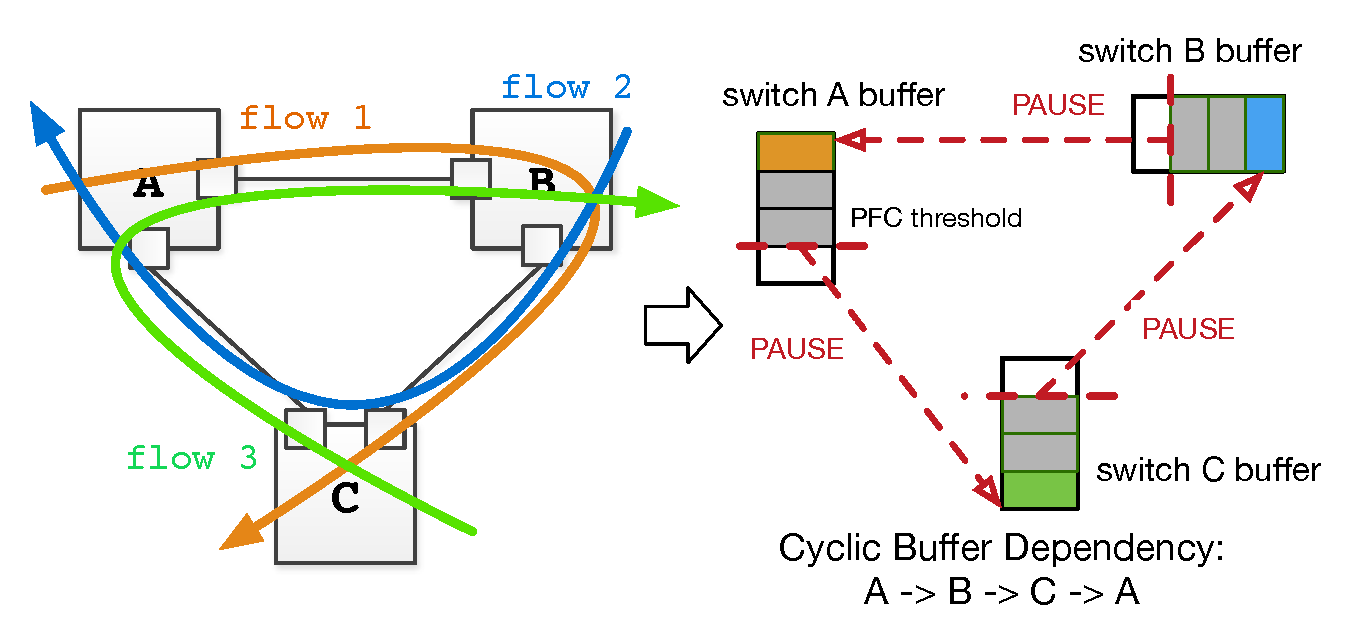
\includegraphics[width=0.45\textwidth] {figs/deadlock}
		\vspace{-1em}
		\caption{A simple (but contrived) example to illustrate CBD formation
		without routing loop.}
		\vspace{-1em}
		\label{fig:basic_deadlock}
\end{figure}

	\section{Background}
\label{sec:background}

We now provide a brief primer on RDMA, RoCE, the problem of deadlocks and prior
work in this area.

{\bf RDMA and RoCE:} Remote Direct Memory Access (RDMA) technology offers high
throughput, low latency and low CPU overhead, by bypassing end-host networking
stacks. Instead, Network Interface Cards(NICS) transfer data in and out of
pre-registered memory buffers at the two end hosts.  In modern data centers,
RDMA is deployed using RDMA over Converged Ethernet V2 (RoCE)
standard~\cite{roce,rroce}

{\bf PFC:} RoCE needs a lossless L2 layer for optimal performance. This is
accomplished in Ethernet networks using the Priority Flow Control (PFC)
mechanism~\cite{pfc}.  Using PFC, a switch can pause an incoming link when its
ingress buffer occupancy reaches a preset threshold. As long as sufficient
``headroom'' is reserved to buffer packets that are in flight during the time
takes for the PAUSE to take effect, no packet will be dropped due to buffer
overflow~\cite{cisco-whitepaper,dcqcn}. 

The PFC standard defines 8 classes\footnote{Although, only one or two can be
used in practice -- see \S\ref{subsec:pfcheadroom}.}, called priorities~\footnote{The word priority is a
misnomer. There is no implicit ordering among priorities -- they are really just
separate classes.}. Packets in each priority are buffered separately, and PAUSE
messages carry this priority.  When a packet arrives at port $i$ of switch $S$
with priority $j$, it is enqueued in queue $j$ of port $i$. If the queue length
now exceeds the PFC threshold, a pause message (XOFF) is sent to the upstream
switch connected to port $i$. The message carries priority $j$. The upstream
switch then stops sending packets with priority $j$ to switch $S$ on port $i$ until a resume
message (XOFF) with priority $j$ is received.

PFC prevents buffer overflow, but it can lead to deadlocks.

%% Since PAUsing is carried out
%% on a per-ingress port, and not on a per-flow basis, problems such as unfairness
%% and head-of-the-line blocking may occur~\cite{dcqcn}. The PFC standard defines 8
%% classes (called priorities), where packets in class are buffered separately, to
%% mitigate these problems~\cite{dcqcn}. However, sine each priority needs its own
%% dedicated headroom, typically, no more than two or three priorities are
%% used~\cite{rdmaatscale}.

{\bf Deadlock:} Deadlock forms when paused links form a cycle
(Figure~\ref{fig:deadlock_example}). Once formed,
deadlock is ``permanent'' in the sense that it will continue to exist even if no
new traffic is injected into the loop. Deadlocks in PFC-based networks (or more
generally, in credit-flow networks) are a well-known problem. It is not merely a
theoretical problem -- it has been reported in practice~\cite{rdmaatscale}.

It is well known that Circular Buffer Dependency (CBD) is a {\em necessary}
condition for deadlock formation~\cite{tcp-bolt,hu2016deadlocks}. {\em
Sufficient} condition for deadlock formation in PFC networks have yet to be
fully understood~\cite{hu2016deadlocks}. 

{\bf Prior work on deadlock avoidance:} Prior work on deadlock management falls
in two categories: deadlock avoidance, or deadlock detection and resolution. Our
focus in this paper is on deadlock avoidance.  Since {\em sufficient} conditions
for deadlock formation are not well characterized, deadlock avoidance schemes
focus on preventing CBD for occurring. This is done either by limiting or
modifying routing~\cite{tcpbolt} to avoid CBD, or by careful buffer
management~\cite{xxx}. 

However, these schemes fail to meet one or more of the three key challenges:
$(i)$ they cannot be deployed with existing routing, or, $(ii)$ they do not deal
with dynamic nature of data center networks, or, $(iii)$ they require excessive
switch buffers or number of priorities. 

We now describe these three challenges in more detail. See \S\ref{sec:related}
for a detailed review of prior work.

%% Prior work on deadlock formation fails to meet the three challanges: first, they
%% do not work with To avoid such deadlocks, {\em deadlock-free
%% routing}~\cite{tcpbolt} has been proposed. It guarantees that (if the routing
%% configuration is correct,) any traffic does not cause deadlock.
%% 
%% Unfortunately, achieving deadlock-free routing is inefficient, and may not even
%% be viable. Deadlock-free routing is achieved by eliminating Cyclic Buffer
%% Dependency (CBD)~\cite{deadlockfree}.  However, ensuring that there is never any
%% CBD is challenging.
%% 
%% First, deadlock-free routing largely limits the choice of topology. For example,
%% Stephens et al. \cite{tcpbolt} proposes to only use tree-based topology and
%% routing, and shows that it is deadlock-free.  However, there are a number of
%% other datacenter topologies and routing schemes that are not
%% tree-based~\cite{bcube, camcube, jellyfish}, and do not have deadlock-free
%% guarantee.
%% 
%% Second, due to bugs or misconfiguration, deadlock-free routing configuration may
%% turn into deadlock-vulnerable. In fact, recent work has observed a PFC deadlock
%% case in real-world tree-based datacenter\cite{rdmascale}, caused by the
%% (unexpected) flooding of lossless class traffic.  Furthermore, there are
%% multiple reports of routing loops due to misconfiguration in today's production
%% datacenters~\cite{everflow, libra}. If lossless traffic encounters any of these
%% loops, CBD is unavoidable.  
%% 
%% Indeed, a recent paper~\cite{hu2016deadlocks} argued that preventing CBD is
%% quite difficult, so instead we should focus on defining and preventing
%% ``simpler''{\em sufficient} conditions to avoid deadlock. 
%% 
%% In this paper, we show that it is indeed possible to prevent CBD, in any
%% topology, without any changes to the underlying routing protocol, using existing
%% data center hardware. 





	%\vspace{-0.1in}
\section{Challenges}
\label{sec:challenges}

\subsection{Work with existing routing protocols and hardware}
\label{sec:incremental} Data center routing protocols have to satisfy a variety
of complex requirements regarding fault tolerance, and
security~\cite{beckett2016don}.  Operators also invest heavily in  tools and
technologies to monitor and maintain their networks; and these tools are
tailored for the routing protocols that are already deployed.  Thus, operators
are unwilling to deploy a brand-new routing
protocols like~\cite{dally,duato93,dally93,sancho2004,flich2012survey,lash,wu2003fault,glass,duato2001,domke2011,puente1999,dfedst16}
or hardware just for deadlock avoidance --  especially when RoCEv2 itself can be
deployed without any changes to routing\footnote{RoCEv2 packets are encapsulated
in standard UDP packets.}! 

\subsection{Data center networks are dynamic}\label{sec:reroute}

A deadlock avoidance scheme that works with existing routing infrastructure must
address the issue that most routing schemes are dynamic -- paths change in
response to link failures or other events.

Figure~\ref{fig:basic_clos} shows a simplified (and small) version
of network deployed in our data center, with commonly used up-down routing (also
called valley-free~\cite{qiu2007toward}) scheme.  In up-down routing, a packet first
goes UP from the source server to one of the common ancestor switches of the
source and destination servers, then it goes DOWN from the common ancestor to
the destination server.  In UP-DOWN routing, the following property holds: when
the packet is on its way UP, it should not go DOWN; when it is on its way DOWN,
it should not go UP. Thus, with up-down routing, there can be no CBD and hence
no deadlock.

However, packets can deviate from the UP-DOWN paths due to many reasons,
including link failures, port flaps etc., which are quite common in data
center networks~\cite{netpilot,f10}. When the up-down property is violated,
packets ``bouncing'' between layers can cause
deadlocks~\cite{shpiner2016unlocking}. See
Figure~\ref{fig:clos_1_bounce}.

In our data centers, we see hundreds of violations of up-down routing per
day. Such routes can persist for minutes or even longer. Overall, we estimate
that $0.001\%$ of the traffic is routed over such paths. This may sound tiny,
but given that our network carries exabytes of traffic per day, the absolute
volume of traffic affected by such routing is in tens of terabytes. This makes
the threat of deadlocks, as discussed
in\cite{rdmaatscale,shpiner2016unlocking,hu2016deadlocks} quite real.

\subsection{Limited number of lossless queues}
\label{subsec:pfcheadroom}

One idea to solve deadlock is to assign dynamic priority to packets. The
priority of a packet increases as the packet approaches its destination
~\cite{karol2003prevention}.  Such a design requires as many priorities as the largest 
path length in the network.  The problem with this idea is that the PFC standard
supports only 8 priority classes. Worse yet, commodity switches can
realistically support fewer than 8 lossless classes.  The problem is that  to
guarantee the lossless property, a switch needs to reserve certain amount of
{\it headroom} per port, per lossless queue.

The headroom is needed to absorb the packets that are in flight during the time
it takes for the PAUSE message to take effect.
The headroom size depends on many factors, including length
of cables. See Appendix \ref{APPHEADROOM} for details.  A
32-port 40GbE Ethernet switch needs to reserve 2.76MB of headroom to support one
lossless queue on all ports. A commodity switch like this typically has
12MB total buffer\footnote{The memory used to build switch buffers needs to be
extremely fast (e.g. 32x40GB switch needs memory that can support read/write
speeds of 1.28 Tbps), and hence is very expensive.}, so 23\%
of the total switch buffer is needed to support just one lossless priority.

While this headroom is sufficient to avoid packet drops, in practice, we use a
slightly larger value to avoid buffer under-flow when the receiver un-pauses the
sender.  Furthermore, we need to reserve buffers for non-RDMA (i.e. lossy)
traffic, which is still the dominating traffic in data centers. With these
constrains, the current commodity switches can typically support just two or
three lossless classes~\cite{rdmaatscale}.

New switching ASICs may be able to support more lossless queues by adding more
memory, using smaller cell size (64-byte) and by reducing the pause frame
response time. But even these are not expected to support more than four or five
lossless queues. Hence the solutions that require a large number of lossless
queues are not practical.

We now describe how \sysname{} addresses these challenges.

	%\vspace{-0.1in}
\section{Achieving Optimal Solution for Structured Topology}\label{sec:specific}

\subsection{Caveats of the Generic Greedy Solution}

\begin{enumerate}
	\item It does not always yield optimal results in terms of number of lossless queues, e.g., in Fat-tree.
	
	\item It requires $M*N$ lossless queues, where $M$ is the number of lossless application classes, 
	$N$ is the number of lossless queues required by each application class. In fact, we may reduce it to $M+N-1$.
 
\end{enumerate}

\subsection{Optimizing Fat-Tree Topology}

\subsection{Optimizing BCube Topology}

\subsection{High-level Takeaways}


\if 0
\subsubsection{Definition of switch functions}
 
\begin{enumerate}
	
	\item \textbf{Packet scheduling function of VIQs $f^{in}_{sche}$:} This is the switch function to decide which packet currently queued in some VIQ $q_{in}^{i}$ to be processed at first. Formally, this function can be expressed as follows. 
	\begin{align} \label{eqn:inschedule}
	 f^{in}_{sche}: q_{in}^{i} \longrightarrow p \in q_{in}^{i}
	\end{align}
	
	\item \textbf{Packet scheduling function of VEQs $f^{out}_{sche}$:} This is the switch function to decide which packet currently queued in some VEQ $q_{out}^{i}$ to be processed at first. Formally, this function can be expressed as follows. 
	\begin{align} \label{eqn:outschedule}
	f^{out}_{sche}: q_{out}^{i} \longrightarrow p \in q_{out}^{i}
	\end{align}
	
	\item \textbf{Packet forwarding function $ f_{fwd}$:} This is the switch function to forward a packet from a VIQ to a VEQ. Formally, this function can be expressed as follows. 
	\begin{align} \label{eqn:fwd}
	 &	f_{fwd}: (q_{in}^{i_1,j}, q_{out}^{i_2,j}, p\in q_{in}^{i_1,j})  \longrightarrow \nonumber \\
	 	&\begin{cases}
	 	 q_{in}^{i_1,j}=q_{in}^{i_1,j}-\{p\},  \text{current node is destination of } p,\\
	     q_{out}^{i_2,j}=q_{out}^{i_2,j}\cup\{p\}, \text{otherwise.} 
	 	\end{cases}
	\end{align}
	
	
	\item \textbf{Packet transmission function $ f_{trans}$:} This is the switch function to send a packet from the VEQ of current network device to the VIQ of the immediate downstream device. Formally, this function can be expressed as follows:
	\begin{align} \label{eqn:trans}
	f_{trans}: &(q_{in}^{i_1, j}, q_{out}^{i_2, j}, q_{in}^{i_3, j+1}, p\in q_{in}^{i_1,j}\cap q_{out}^{i_2,j})  \longrightarrow  \nonumber \\
 &	(q_{in}^{i_1,j}=q_{in}^{i_1,j}-\{p\}, q_{out}^{i_2,j}=q_{out}^{i_2,j}-\{p\}, \nonumber \\ 
 &	 q_{in}^{i_3,j+1}=q_{in}^{i_3,j+1}\cup\{p\}),  \nonumber \\
 & \text{if } p_{ttl} > 0   
 	\end{align}
 	\begin{align} 
 	f_{trans}: &(q_{in}^{i_1, j}, q_{out}^{i_2, j}, p\in q_{in}^{i_1,j}\cap q_{out}^{i_2,j})  \longrightarrow  \nonumber \\
 	&(q_{in}^{i_1,j}=q_{in}^{i_1,j}-\{p\}, q_{out}^{i_2,j}=q_{out}^{i_2,j}-\{p\}), \nonumber \\ 
 	& \text{if } p_{ttl} =0
	\end{align}
	Note that here  $q_{in}^{i_1, j}$ and $q_{out}^{i_2,j}$ are two queues belonging to the same network node, while $q_{in}^{i_3, j+1}$ is a queue belonging to an immediate downstream network node.
\end{enumerate}


\subsubsection{Assumptions}

Let $t_{cost}(f)$ be the time cost of performing switch function $f$. In the following part, we list several assumptions we make in our proof.

\begin{enumerate}
	\item \textbf{PFC threshold is no smaller than maximum transmission unit (MTU):} Formally, we have $t_{PFC}\ge s_{MTU}$.
	
	\item \textbf{Finite packet scheduling time:} We assume that packet scheduling functions can decide the next packet to be processed within finite time. Formally, $f^{in}_{sche}$ and $f^{out}_{sche}$ should satisfy the following constraints at any network node:
		\begin{align} 
    	t_{cost}(f^{in}_{sche}(q_{in}^{i})) < \infty ,1\leq i \leq n \label{eqn:schecon1}\\
	    t_{cost}(f^{out}_{sche}(q_{out}^{i})) < \infty, 1\leq i \leq n \label{eqn:schecon2}
		\end{align}
		
	\item \textbf{No selection of duplicated packet:} the packet scheduling function $f^{in}_{sche}$ will not select the same packet twice. Formally, 
		\begin{align} \label{eqn:nodupschedule}
		f^{in}_{sche}: \quad& q_{in}^{i_1} \longrightarrow p \in q_{in}^{i_1}, \nonumber \\
		\mbox{Subject to}: \quad&1\leq i_2 \leq n, \forall p\prime \in q_{out}^{i_2}, p \neq p\prime .
		\end{align}
		
	\item \textbf{Prefering non-paused packet:} We assume $f^{out}_{sche}$ will always prefer non-paused packets over paused packets.
		
	\item \textbf{Finite packet forwarding time:} We assume that any packet can be forwarded from a VIQ to a VEQ within finite time. Formally, $f_{fwd}$ should satisfy the following constraint:
	    \begin{align} \label{eqn:fwdcon}
		t_{cost}(f_{fwd}((q_{in}^{i_1,j}, q_{out}^{i_2,j}, p\in q_{in}^{i_1,j}))) < \infty, \nonumber \\
		1\leq i_1, i_2 \leq n
		\end{align}
		
	\item \textbf{Finite packet transmission time when no PFC pause:} We assume that any packet can be sent to the VIQ of next hop within finite time when the priority class of the packet is not paused by the immediate downstream device. Formally, $f_{trans}$ should satisfy the following constraint:
	
	\begin{align} \label{eqn:transcon}
	t_{cost}(f_{trans}(q_{in}^{i_1, j}, q_{out}^{i_2, j}, q_{in}^{i_3, j+1}, p\in q_{in}^{i_1,j}\cap q_{out}^{i_2,j}))= \nonumber \\
	\begin{cases}
	<\infty, &\quad |q_{in}^{i_3,j+1}|< t_{PFC}\\
	\infty, &\quad\text{otherwise.} \ 
	\end{cases}
	\end{align}
	
    \end{enumerate}
    
    
   \subsubsection{Network Buffer State}
   
   \textbf{Buffer state:} we use a $2n$ dimensional vector  to represent the buffer state of a network node $u$ as follows: 
   \begin{align}
   BS_u=<q_{in}^{1}, \dots, q_{in}^{n}, q_{out}^{1}, \dots,q_{out}^{n}> \nonumber 
   	\end{align}
   	$BS_u(t)$ is the buffer state of node $u$ at time $t$.
   
   Let $N(V,E)$ be the network topology, where $V$ is the set of network nodes and $E$ is the set of network links. We represent the buffer state of netwrok $N$ (denoted as $BS_N$) as follows:
   \begin{align}
   BS_N=<BS_{u_1},\dots,BS_{u_i},\dots>,\forall u_i \in V \nonumber 
   \end{align}
   $BS_N(t)$ is the buffer state of network $N$ at time $t$.
   
   \textbf{Legal buffer state:} We say $BS_u$ is a legal buffer state for node $u$ when the following two conditions are satisfied:
   \begin{align} \label{eqn:legalstatecon}
    |q_{in}^{i}|<\infty\quad  \text{and}\quad   |q_{out}^{i}|<\infty, \quad 1\leq i \leq n
%    |q_{in}^{i,j}|\leq t_{PFC}, \quad 1\leq i \leq n, 1\leq j \leq k \label{eqn:legalstatecon2}
   \end{align}
   
   We say $BS_N$ is a legal buffer state when the buffer state of every node in $N$ is legal.
   
   \textbf{Empty buffer state:} We say $BS_u$ is an empty buffer state when the following condition is satisfied:
    \begin{align} \label{eqn:emptystatecon}
    |q_{in}^{i}|=0\quad  \text{and}\quad   |q_{out}^{i}|=0, \quad 1\leq i \leq n 
    \end{align}
    
    We say $BS_N$ is a empty buffer state when the buffer state of every node in $N$ is empty. Specially, we denote the empty buffer state of network $N$ as $BS^0_N$.
    
  \textbf{Deadlocked buffer state:} $\forall t< \infty$, we say $BS_N(t)$ is a deadlocked buffer state if the following condition is met when no new packets are injected into the network since $t$:
  \begin{align} \label{eqn:deadlockstatedef}
  \exists \text{ finite } t_0 > t, \quad \forall t_1>t_0, \nonumber\\
  BS_N(t_1)\equiv BS_N(t_0) \quad \text{and} \quad BS_N(t_0) \neq BS^0_N.
  \end{align}
    
\fi 0

    %     \textbf{Lemma 1}: for arbitrary non-deadlocked buffer state $BS_N(t)$, when no new packets are injected into the network since $t$, there exists a finite $t_0>t$, $BS_N(t_0)=BS^0_N$.
    %     
    %      \textbf{Proof}: Assuming that there does not exist a finite $t_0>t$, $BS_N(t_0)=BS^0_N$. As $BS_N(t)$ is a non-deadlocked buffer state, according to Equation~\ref{eqn:deadlockstatedef}, $BS_N(t)$ will not converge into any fixed non-empty buffer state. 
    %      
    %      Let $BS_N(t_1), \dots, BS_N(t_i), \dots$ be the buffer states $BS_N(t)$ will transition to in sequence since $t$. Let $Sum_{TTL}(BS_N(t))$ be the sum of TTL values of all packets 
    %      
    %      We consider any transition from $BS_N(t_i)$ to $BS_N(t_{i+1})$, $i>0$,
    %      
    %      \textbf{}
    
%\textcolor{red}{To be added.}

%In this part, we will prove that our solution can ensure a \textit{lossless} network and at the same time is \textit{deadlock-free} when the following four assumptions are met.
%
%\textbf{Assumption 1}: There is no transmission or processing errors at all the network nodes.
%
%\textbf{Assumption 2}: PFC PAUSE/RESUME messages can take effect immediately at the corresponding upstream node, i.e., there is no link delay and processing delay.
%
%\textbf{Assumption 3}: The scheduling algorithm of any VIQ is deadlock-free: for any given time $t$, any packet $p$ queued in arbitrary $q_{in}^{i,j}$, $1\leq i \leq n$, $1 \leq j \leq k$, can be forwarded to the destined VEQ within some finite time since $t$.
%
%\textbf{Assumption 4}: The scheduling algorithm of any VEQ is deadlock-free: for any given time $t$, any packet $p$ queued in arbitrary $q_{out}^{i,j}$, $1\leq i \leq n$, $1 \leq j \leq k$, can be forwarded to next hop's VIQ via output port $i$ within some finite time since $t$, as long as two conditions are met: 1) $q_{out}^{i,j}$ is not paused by PFC PAUSE message since $t$; 2) VEQ $i$ does not receive any new packets since $t$.
%
%\textbf{Claim 1}: The TTL based buffer management scheme can work with the modified PFC mechanism to ensure a lossless network.
%
%\textbf{Claim 2}: The network is deadlock-free after applying the TTL based buffer management scheme and the modified PFC mechanism.
%
%To prove the above two claims, we first present two lemmas.
%
%\textbf{Lemma 1}: The priority class $\lambda_p$ of a packet $p$ buffered at a given node always satisfies $\lambda_p \leq d$.
%
%\textit{Proof}: As a packet with TTL value equal to 0 will be dropped by the received node, we have $ttl_i \geq 0$. Then we have $\lambda_p = ttl_0 - ttl_i \leq ttl_0 - 0 = d$.
%
%\textbf{Lemma 2}: If we stop injecting new packets into the network since some time $t_0$, arbitrary $q_{out}^{i,j}$, $1\leq i \leq n$, $1 \leq j \leq k$, will become empty within some finite time since $t_0$. 
%
%\textit{Proof}: We use induction on $\lambda_p$ to prove the lemma. First, we consider $\lambda_p=d$. 
%
%Under our modified PFC mechanism, pacekts in $q_{in}^{i,j}$ of some node are only possible to pause the packet transmission of the immediate upstream node on priority class $j$-$1$.  So packets in any $q_{out}^{i,j}$ of one node are only possible to be paused by the packets of higher priority class at some immediate downstream node. According to Lemma 1,  $q_{out}^{i,d}$ is the queue of highest priority class among all the non-empty queues. Hence packets in $q_{out}^{i,d}$ will not be paused by PFC PAUSE messages. 
%
%In the next, we prove by contradiction that any packet in $q_{out}^{i,d}$ can get drained within some finite time since $t_0$. We first assume that there exists a packet $p$ in $q_{out}^{i,d}$ which cannot get drained within some finite time since $t_0$. According to Assumption 4, if the following two conditions are met, packet $p$ will get drained within some finite time: (1) $q_{out}^{i,d}$ is not paused by PFC PAUSE messages; and (2) there exists a finite time $t_1>t_0$,  since which no new packets will be forwarded to VEQ $i$. The first condition is already met. To make our assumption valid, we can conclude that there does not exist a finite time $t_1>t_0$,  since which no new packets will be forwarded to VEQ $i$.
%
%As no new packets are injecting into the network since $t_0$, the number of packets remaining in the network is finite (denoted as $N_p$). Further, any packet traversing more than $d$ hops in the network will be dropped. Therefore, the number of packets to be forwarded to VEQ $i$ since $t_0$ is finite (no larger than $N_p*d$). 
%
%Let $t_1$ be the time at which the last packet is forwarded to VEQ $i$. $t_1$ must be finite as there are only finite number of packets to be forwarded to VEQ $i$. This contradicts with the conclusion that there does not exist a finite time $t_1>t_0$,  after which no new packets are forwarded to VEQ $i$. So our previous assumption is not valid. Then we can conclude that any packet in $q_{out}^{i,d}$ can get drained within some finite time since $t_0$.
%
%Since (1) any packet in $q_{out}^{i,d}$ can get drained within some finite time since $t_0$ and (2) the number of packets to be forwarded to VEQ $i$ since $t_0$ is finite, $q_{out}^{i,j}$ will become empty within some finite time since $t_0$. 
%
%Next, we show that the lemma holds for $\lambda_p=d-1$. After $q_{out}^{i,j}$ becomes empty at all the nodes, $q_{out}^{i,d-1}$ becomes the queue of highest priority class among all the non-empty queues. Following the same analysis, we can know that $q_{out}^{i,d-1}$ will become empty within some finite time since $t_0$. This completes proof of the lemma.
%
%
%\textbf{Proof of Claim 1}: Let $b_j$ be the buffer size of the $j$-$th$ buffer partition. At every switch and every server, we set the PFC threshold of priority class $j$ as $b_j-n*m_{max}$.
%
%At any given time $t$, we consider packet $p$ in the head of arbitrary $q_{out}^{i,j}$, $1\leq i \leq n$, $1 \leq j \leq k$. 
%
%Case 1: $q_{out}^{i,j}$ is not paused by PFC PAUSE messages at time $t$. According to the PFC threshold, at the immediate downstream node, the remaining buffer size of the ($j$+$1$)-$th$ buffer partition will be no smaller than $n*m_{p}$, where $n$ is the number of switch ports and $m_{p}$ is the maximum packet size.  In the worst case, when packet $p$ is being sent to the immediate downstream node, other $n$-$1$ packets are being sent to the same node over different input ports at the same time. As the remaining buffer is large enough to accommodate all these $n$ packets, packet $p$ will not be dropped.
%
%case 2: $q_{out}^{i,j}$ is paused by PFC PAUSE messages at time $t$. In this case, packet $p$ will not be dropped as it is paused.
%
%In the above analysis, the consideration of packet $p$ and time $t$ is arbitrary, so no packet will be dropped at any node under our solution. So our solution can ensure a lossless network when properly setting the PFC threshold.
%
%\textbf{Proof of Claim 2}: For arbitrary given time $t$, in order to know whether the network is already in a state of deadlock, we can stop the injection of new packets into the network at time $t$, and observe whether all the packets remaining in the network can get drained within some finite time. 
%
%According to Lemma 2, under our TTL-based buffer management scheme, if we stop the injection of new packets into the network at time $t$, all VEQs will become empty within some finite time since $t$. According to Assumption 3, no packet will be permanently buffered in the VIQs. So packets in VIQs can also get drained within some finite time. Therefore, all the packets remaining in the network can get drained within some finite time. 
%
%Based on the above discussion, our TTL-based buffer management scheme is deadlock-free.


	\section{Generalizing \sysname{}}
\label{sec:generic}

We begin by  formalizing the description of the tagging system using notation in
Table~\ref{tab:symbols}.

Let $A_i$ represent a unique ingress port in the network, {\em i.e.,} switch
$A$'s $i^{th}$ ingress port.  We use a {\em tagged graph} $G(V,E)$ to uniquely
represent a tagging scheme.  Given a tagging scheme, the {\em tagged graph}
$G(V,E)$ is defined as:

\begin{enumerate}
\item $G$ contains a node, $(A_i, x)$, {\em iff.} port $A_i$ may receive packets with tag $x$, and these packets must
be lossless. $V$ is the set of all such nodes.

\item $G$ contains an edge $(A_i, x)\rightarrow(B_j, y)$ {\em iff.} switch $A$ and $B$ are
connected, {\em and} switch $A$ may change a packet's tag from $x$ to $y$ before sending to $B$ (the case $x=y$ also counts).
$E$ is the set of all such edges.

\end{enumerate}

Given a tag $k$, we also define $\{G_k\}$, with vertices $V(G_k)$ and edges
$E(G_k)$:
$$V(G_k) = \{(A_i, k) | \forall A, i\} $$
$$E(G_k) = \{v_0 \rightarrow v_1 | \forall v_0, v_1 \in V(G_k),  v_0 \rightarrow v_1 \in E(G)\} $$
Each tag $k$ is mapped to a unique lossless priority.

Each node has a rule to match on a tag on an ingress port, and assign the packet
to corresponding lossless queue.  In addition, each edge corresponds to a switch
action of setting the tag for the next hop at the egress port.

\begin{table}[t]
\small
\centering
\begin{tabular}{|c|c|}
\hline
Symbol & Description \\ \hline
$A_i$ & Switch $A$'s $i^{th}$ ingress port  \\ \hline
$(A_i, x)$ & A node in tagged graph \\ \hline
$(A_i, x)\rightarrow(B_j, y)$ & A tagged edge \\ \hline
$V$ & All tagged nodes  \\ \hline
$E$ & All tagged edges \\ \hline
$G(V, E)$ & Tagged graph \\ \hline
$G_k$ & Partition of $G(V,E)$ for priority $k$ \\ \hline
\end{tabular}
\caption{Notations in the formalized description.}
\label{tab:symbols}
		\vspace{-1em}
\end{table}

If a packet arrives at $A_i$ with tag $x$, and is destined for port $B_j$, and
there is no corresponding edge in $G(V,E)$, it means that the packet has
traversed on a path that is not in ELP.  Such packets are assigned a special
tag, and all switches assign this tag to lossy priority\footnote{This rule is
always the last one in the TCAM rule list, acting as a safeguard to avoid
unexpected buffer dependency.  See \S\ref{sec:implementation}.}.

In the rest of the section, we will describe how to generate the tagging graph
-- i.e. the tagging rules. But first, we prove that the tagging scheme described
by such a graph is deadlock free, as long as the graph meets two requirements.

\begin{enumerate}

		\item  Any $G_k$ for $G$ {\em must not} have a cycle.  This is
				because each edge in $G_k$ is essentially a buffer dependency --
				whether $A_i$ can dequeue packets depends on whether $B_j$ has
				paused it. A cycle in $G_k$ means cyclic buffer
				dependency.
		\item There must be no link going from
				$G_x$ to $G_y$ if $x>y$.  This means we enforce the order of
				$G_x$ and $G_y$.
\end{enumerate}
These requirements are essentially generalization of the properties
discussed in \S\ref{subsec:specific_deadlock_free}.
\begin{theorem}
Any tag system, defined by $G(V,E)$, that satisfies the above two requirements is deadlock-free.
\end{theorem}

\begin{proof}
We prove by contradiction. Suppose there exists a tag system,
whose $G(V,E)$ satisfies the above two requirements, but is not deadlock-free. This means
$G(V,E)$ has a cycle $v_0 \rightarrow v_1 \rightarrow ... \rightarrow v_0$. If
traffic that covers all hops in the cycle, the cycle leads into a CBD and can form deadlock.

\textbf{Case 1:} All the nodes in the cycle has the same tag $t$. According to
the first requirement, $G_t$ does {\em not} have a cycle. Contradicted.

\textbf{Case 2:} The nodes in the cycle have at least two different tags, $t_0$ and $t_1$.
Without loss of generality, we assume $t_0 < t_1$, and $v_i$ has tag $t_0$, $v_j$
has tag $t_1$. Because $v_i$ and $v_j$ belongs to a circle, there must exists
a path going from $v_j$ to $v_i$. Since $t_0 < t_1$, along the path there must exist
a hop where the tag decreases. However, according to the second requirement, such a hop
cannot exist. Contradicted.

Case 1 and Case 2 cover all possible scenarios. Thus, we conclude that there does not
exist a $G(V,E)$ that satisfies the two requirements but is not deadlock-free.
\end{proof}
We now describe the algorithm to generate $G(V,E)$ for any given topology, and
the ELP set.
\subsection{Generating $G(V,E)$}
\begin{figure*}[t]
	\centering
		\subfloat[short for lof][Topology and ELP set.] {
		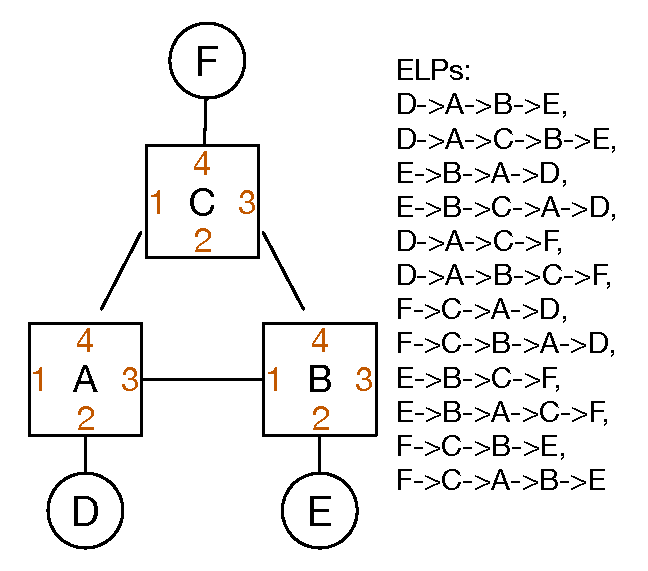
\includegraphics[width=0.26\textwidth] {figs/alo_walkthrough_a}
	}
	\subfloat[short for lof][Output tagged graph Algorithm~\ref{alg:ttl}.]{
		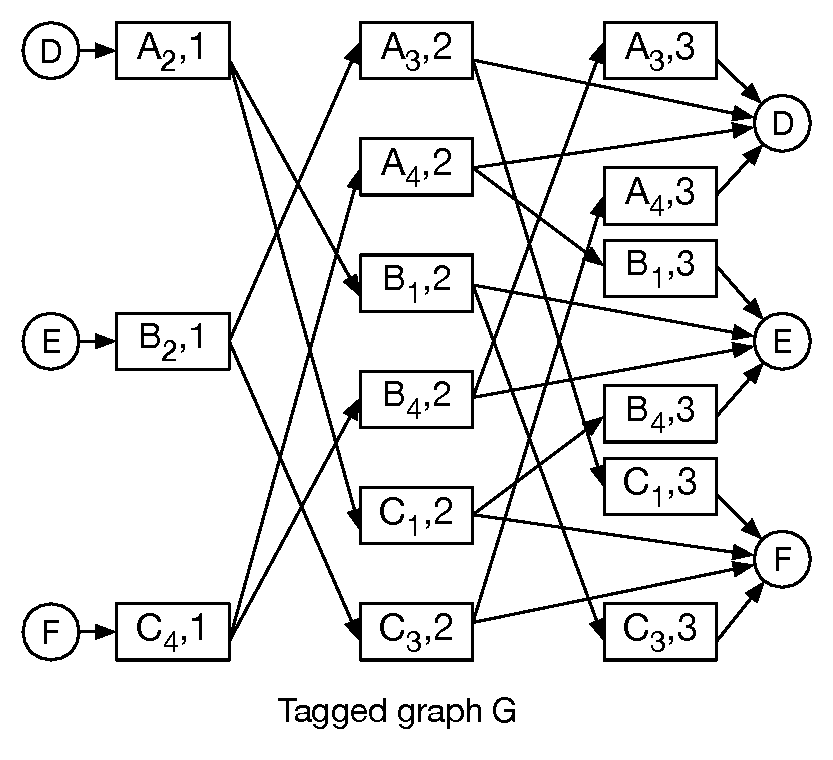
\includegraphics[width=0.27\textwidth] {figs/alo_walkthrough_b}
	}
	\subfloat[short for lof][Output tagged graph by Algorithm~\ref{alg:greedy}.]{
	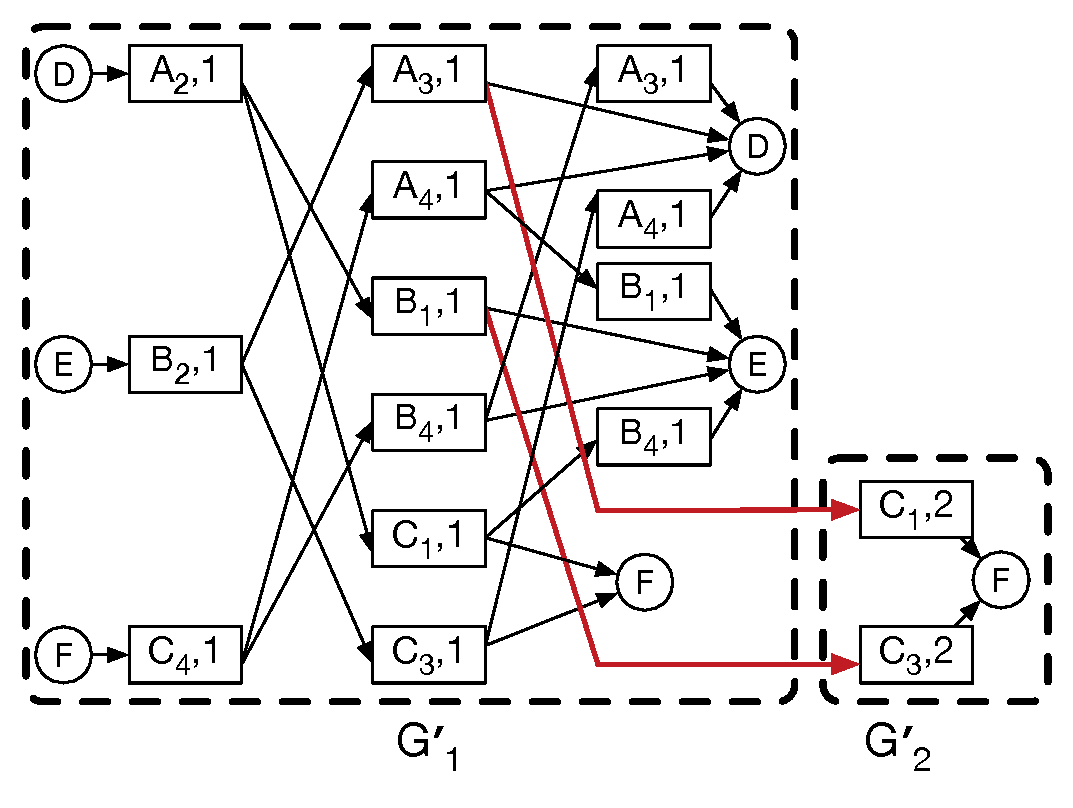
\includegraphics[width=0.34\textwidth] {figs/alo_walkthrough_c}
}
	\caption{Walk-through example of the algorithms.}\label{fig:three_node}
\end{figure*}

\begin{table*}[t]
    \footnotesize
	\centering
	\begin{tabular}{lll}
		\begin{tabular}{|r|r|r|r|}
			\hline
			Tag&  Ingress& Egress & \textcolor{red}{Newtag} \\
			\hline
			\hline
			1 & 2 & 3 & \textcolor{red}{2} \\
			\hline
			1 & 2 & 4 & \textcolor{red}{2} \\
			\hline
			2 & 3 & 2 & \textcolor{red}{3} \\
			\hline
			2 & 3 & 4 & \textcolor{red}{3} \\
			\hline
			2 & 4 & 2 & \textcolor{red}{3} \\
			\hline
			2 & 4 & 3 & \textcolor{red}{3} \\
			\hline
			3 & 3 & 2& \textcolor{red}{4} \\
			\hline
			3 & 4 & 2 & \textcolor{red}{4} \\
			\hline
			others & others & others & \textcolor{red}{lossy tag} \\
			\hline
			\multicolumn{4}{c}{(a) rules installed in A} \\
		\end{tabular}
		&
		\begin{tabular}{|r|r|r|r|}
			\hline
			Tag&  Ingress& Egress & \textcolor{red}{Newtag} \\
			\hline
			\hline
			1 & 2 & 1 & \textcolor{red}{2} \\
			\hline
			1 & 2 & 4 & \textcolor{red}{2} \\
			\hline
			2 & 1 & 2 & \textcolor{red}{3} \\
			\hline
			2 & 1 & 4 & \textcolor{red}{3} \\
			\hline
			2 & 4 & 1 & \textcolor{red}{3} \\
			\hline
			2 & 4 & 2 & \textcolor{red}{3} \\
			\hline
			3 & 1 & 2& \textcolor{red}{4} \\
			\hline
			3 & 4 & 2 & \textcolor{red}{4} \\
			\hline
			others & others & others & \textcolor{red}{lossy tag} \\
			\hline
			\multicolumn{4}{c}{(b) rules installed in B} \\
		\end{tabular}
		&
		\begin{tabular}{|r|r|r|r|}
			\hline
			Tag&  Ingress& Egress & \textcolor{red}{Newtag} \\
			\hline
			\hline
			1 & 4 & 1 & \textcolor{red}{2} \\
			\hline
			1 & 4 & 3 & \textcolor{red}{2} \\
			\hline
			2 & 1 & 3 & \textcolor{red}{3} \\
			\hline
			2 & 1 & 4 & \textcolor{red}{3} \\
			\hline
			2 & 3 & 1 & \textcolor{red}{3} \\
			\hline
			2 & 3 & 4 & \textcolor{red}{3} \\
			\hline
			3 & 1 & 4 & \textcolor{red}{4} \\
			\hline
			3 & 3 & 4 & \textcolor{red}{4} \\
			\hline
			others & others & others & \textcolor{red}{lossy tag} \\
			\hline
			\multicolumn{4}{c}{(c) rules installed in C} \\
		\end{tabular}
	\end{tabular}
	\caption{Tag rewriting rules under Algorithm~\ref{alg:ttl} (tag ``4'' will only appear on destination servers).}
	\label{table:tagging_table}
\end{table*}

As in \S\ref{sec:specific}, we will first design a tagging scheme that avoids
deadlock, then combine tags to reduce the number of required lossless queues.
For general graph without structure information, a straightforward tagging
system is to monotonically increase the tag (thus, the priority) at every hop,
as described in Algorithm~\ref{alg:ttl}.

\begin{algorithm}[t]
	\small
    \KwIn{Topology and $ELP$}
	\KwOut{A tagged graph $G(V, E)$}
	$V \gets Set()$\;
	$E \gets Set()$\;
	\For{each path $r$ in $ELP$} {
		$tag \gets 1$\;
		\For{each hop $h$ in $r$} {
			$V \gets V \cup \{(h, tag)\}$\;
			$E \gets E \cup \{lastHop\rightarrow(h, tag)\}$\;
			$tag \gets tag+1$\;
		}
	}
	\Return{$G(V, E)$}\;
    \caption{A brute-force tagging system that decreases the tag by one on every hop.}
	\label{alg:ttl}
\end{algorithm}

It is easy to verify that the graph generated by this algorithm meets the two
requirements specified earlier, and thus it guarantees deadlock freedom.
Figure~\ref{fig:three_node} shows a small example, including the topology, the
ELP set, the generated graph, and the corresponding rule
lists for each node.

Of course, with just this basic algorithm, we may end up with too many tags
(i.e. lossless priorities) -- in fact, as many as the longest path length in
lossless routes. This is why we need three lossless priorities for
the simple example in Figure~\ref{fig:three_node}(b). In a three-layer Clos
network, the longest up-down path has 5 hops, so Algorithm~\ref{alg:ttl} will use 5
priorities just to support up-down routing. We now show how to combine tags to
reduce the number of lossless queues needed.

\subsection{Reducing the number of lossless queues}
%%comment: i do not see the use of micropath before. hence i am recoving it here.
%%comment: need to discuss and decide the smallest tag. I believe it should start from 1. 0 is reserved for lossy.
%%comment: change subspace  to subgraph? it is a dag, hence a graph. but it is not a space.

Algorithm~\ref{alg:greedy} uses a greedy heuristic to combine the tags generated
by Algorithm~\ref{alg:ttl} to reduce the number of lossless queues required.  It
greedily combines as many nodes in $G(V,E)$ as possible into each path segment
under CBD-free constraint. To ensure the monotonic property, we start
from combining the nodes with smallest tag, 1 and proceed linearly to consider
all tags up to $mT$, which is the largest tag number used in $G(V,E)$.

\begin{algorithm}[t]
	\small
    \KwIn{The brute-force tagged graph $G(V, E)$}
	\KwOut{A new tagged graph $G'(V', E')$ that has small $|\{G'_k\}|$}
	Initialize $V'$, $E'$, $V_{tmp}$, $E_{tmp}$ as empty $Set()$\;
	$t' \gets 1$\;
	\For{$t \gets 1$ \textbf{to} $mT$} {
		\For{each $(A_i, t)$ in $V$ whose tag is $t$} {
			$V_{tmp} \gets V_{tmp} \cup \{(A_i, t')\}$\;
			$E_{tmp} \gets E_{tmp} \cup \{$edges of $(A_i, t)$, change $t$ to $t'\}$\;
			\uIf{$G_{tmp}(V_{tmp}, E_{tmp})$ is acyclic} {
				$V' \gets V' \cup \{(A_i, t')\}$\;
				$E' \gets E' \cup \{$edges of $(A_i, t)$, change $t$ to $t'\}$\;
			}
			\Else{
				$V' \gets V' \cup \{(A_i, t'+1)\}$\;
				$E' \gets E' \cup \{$edges of $(A_i, t)$, change $t$ to $t'+1\}$\;
				$V_{tmp} \gets V_{tmp} \backslash \{(A_i, t')\}$\;
				$E_{tmp} \gets E_{tmp} \backslash \{$edges of $(A_i, t')\}$\;
			}
		}
		\uIf{$V'$ contains nodes of tag $t'+1$} {
			$V_{tmp} \gets \{$nodes in $V'$ with tag $t'+1\}$\;
			$E_{tmp} \gets \{$edges in $V'$, both ends have tag $t'+1\}$\;
			$t' \gets t'+1$\;
		}
	}
	\Return{$G'(V', E')$}\;
    \caption{Greedily minimizing the number of tags by merging brute-force tags.}
	\label{alg:greedy}
\end{algorithm}

%\begin{figure}[t]
%	\centering
%	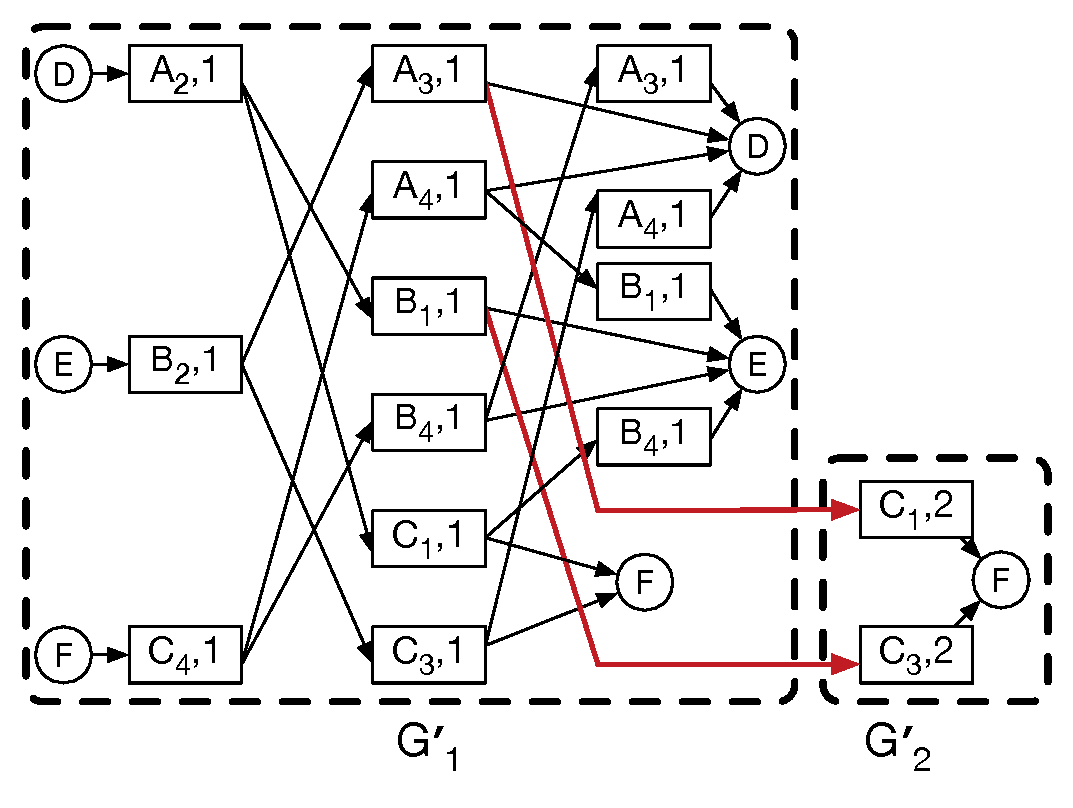
\includegraphics[width=0.48\textwidth] {figs/alo_walkthrough_c}
%	\caption{Algorithm~\ref{alg:greedy} output for the example in Figure~\ref{fig:three_node}.}
%	\label{fig:greedy}
%	\vspace{-1em}
%\end{figure}

\begin{table*}[t]
	\footnotesize
	\centering
	\begin{tabular}{lll}
		\begin{tabular}{|r|r|r|r|}
			\hline
			Tag&  Ingress& Egress & \textcolor{red}{Newtag} \\
			\hline
			\hline
			1 & 2 & 3 & \textcolor{red}{1} \\
			\hline
			1 & 2 & 4 & \textcolor{red}{1} \\
			\hline
			1 & 3 & 2 & \textcolor{red}{1} \\
			\hline
			1 & 3 & 4 & \textcolor{red}{2} \\
			\hline
			1 & 4 & 2 & \textcolor{red}{1} \\
			\hline
			1 & 4 & 3 & \textcolor{red}{1} \\
			\hline
			others & others & others & \textcolor{red}{lossy tag} \\
			\hline
			\multicolumn{4}{c}{(a) rules installed in A} \\
		\end{tabular}
		&
		\begin{tabular}{|r|r|r|r|}
			\hline
			Tag&  Ingress& Egress & \textcolor{red}{Newtag} \\
			\hline
			\hline
			1 & 2 & 1 & \textcolor{red}{1} \\
			\hline
			1 & 2 & 4 & \textcolor{red}{1} \\
			\hline
			1 & 1 & 2 & \textcolor{red}{1} \\
			\hline
			1 & 1 & 4 & \textcolor{red}{2} \\
			\hline
			1 & 4 & 1 & \textcolor{red}{1} \\
			\hline
			1 & 4 & 2 & \textcolor{red}{1} \\
			\hline
			others & others & others & \textcolor{red}{lossy tag} \\
			\hline
			\multicolumn{4}{c}{(b) rules installed in B} \\
		\end{tabular}
		&
		
		\begin{tabular}{|r|r|r|r|}
			\hline
			Tag&  Ingress& Egress & \textcolor{red}{Newtag} \\
			\hline
			\hline
			1 & 4 & 1 & \textcolor{red}{1} \\
			\hline
			1 & 4 & 3 & \textcolor{red}{1} \\
			\hline
			1 & 1 & 3 & \textcolor{red}{1} \\
			\hline
			1 & 1 & 4 & \textcolor{red}{1} \\
			\hline
			1 & 3 & 1 & \textcolor{red}{1} \\
			\hline
			1 & 3 & 4 & \textcolor{red}{1} \\
			\hline
			2 & 1 & 4 & \textcolor{red}{2} \\
			\hline
			2 & 3 & 4 & \textcolor{red}{2} \\
			\hline
			others & others & others & \textcolor{red}{lossy tag} \\
			\hline
			\multicolumn{4}{c}{(c) rules installed in C} \\
		\end{tabular}
		
	\end{tabular}
	\caption{Tag rewriting rules generated by Algorithm~\ref{alg:greedy}.  (Without compression.)}
	\label{table:tagging_table2}
\end{table*}

The new tag $t'$ also starts from 1. In every iteration, we check all nodes with
the same tag value $t$. $V_{tmp}$ and $E_{tmp}$ is the ``sandbox''. For every
node, we add it to $V_{tmp}$ and $E_{tmp}$ and check whether adding it to
$G'_{t'}$ will lead to a cycle within $G'_{t'}$. If not, we re-tag the node to
be $t'$. Otherwise, we re-tag the node to be $t'+1$.  Re-tagging the node to be
$t'+1$ does not cause a cycle in $G'_{t'+1}$, because all nodes in $G'_{t'+1}$
so far have the same old tag of $t$, which means there is no edge between them.
At the end of each iteration, if there are nodes being re-tagged as $t'+1$, we
move on to add nodes into $G'_{t'+1}$ in the next iteration.  This ensures that
the monotonic property will still hold after combination.

In Figure~\ref{fig:three_node}(c) we see Algorithm~\ref{alg:greedy} in action to
minimize the $G(V,E)$ from Figure~\ref{fig:three_node}. We see that the number
of tags is reduced to {\em two}.

\subsection {Analysis}
\label{subsec:caveats}

\para{Algorithm runtime:}. Algorithm~\ref{alg:greedy} is efficient. Recall that
$mT$ is the largest value of tag in $G(V,E)$. Let the number of links in the
original topology be $L$. Then, $G(V,E)$ can have at most have $L \times mT$
nodes.  Each node will be examined exactly once for checking whether $G_{tmp}$
is acyclic.  Checking whether $G_{tmp}$ is acyclic with a newly added node
requires a Breadth-First Search, with runtime complexity of $O(|V_{tmp}| +
|E_{tmp}|)$. $|V_{tmp}|$ is bounded by the number of switches $S$, and
$|E_{tmp}|$ is bounded by the number of links, $L$, in the network.  Therefore,
the total runtime complexity is $O(L \times mT \times (S+L))$. Note that $mT$
itself is bounded by the length of the longest path in $ELP$.

\para{Number of tags:} Algorithm~\ref{alg:greedy} significantly reduces the
number of tags on topology other than Clos. For example, it gives optimal
results for BCube topology without requiring any BCube-specific changes -- a
$k$-level BCube needs $k$ tags to prevent deadlock with default routing. The
results are promising even for unstructured topology like Jellyfish.  For
example, Jellyfish with 2000 nodes require only 3 tags with shortest-path
routing. See \S\ref{sec:eval} for details.

\begin{figure}[t]
	%\vspace{-0.1in}
	\centering
	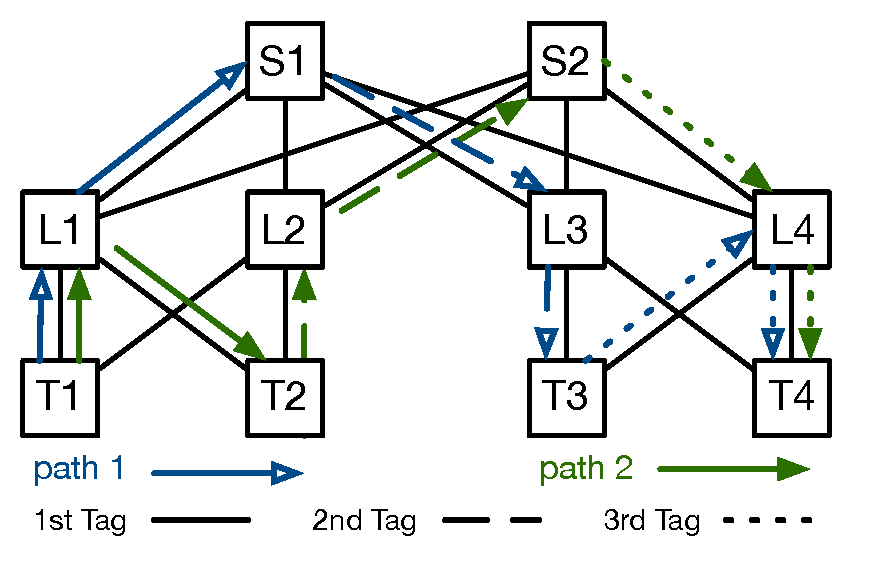
\includegraphics[width=0.48\textwidth] {figs/nonoptimal_example}
	\caption{Algorithm~\ref{alg:greedy} does not output optimal result for Clos with 1-bounce paths.}
	\label{fig:nonoptimal}
	\vspace{-1em}
\end{figure}

\para{Number of rules:} From the conceptual switch model, a switch needs ingress
port number, egress port number, and the current Tag to decide the next Tag.
Hence it seems the number of rules needed per switch is $n(n-1)\times
\frac{m(m-1)}{2}$, where $n$ is the number of switch ports and $m=|G'_{k}|$ is
the number of Tags. We will show in \S~\ref{sec:implementation} that the number
of rules can be compressed to  $n\times \frac{m(m-1)}{2}$, by taking advantage
of the bit masking technique which is widely supported in commodity switching
ASICs. Table~\ref{table:tagging_table2} shows the rules before compression.

\para{Optimality:} Algorithm~\ref{alg:greedy} may not always return the optimal
solution.  Consider the Clos network in Figure~\ref{fig:nonoptimal}.  If ELP
consists of shortest and ``1-bounce'' paths, we know the optimal tagging system
only requires {\em two} lossless queues. However, the greedy algorithm will
output {\em three} lossless queues. The reason is that
Algorithm~\ref{alg:greedy} does not combine bounces that happen when the packet
is going up and when the packet is coming down.

For example, as shown in Figure~\ref{fig:nonoptimal}, the bounce of green flow
will force the algorithm to create a new tag for the first two hops,
since the third hop, which is a bouncing hop, may lead to CBD.  However, the
orange flow bounces at the last two hops and will force the algorithm to create
another new tag. Thus, the algorithm generates three tags, requiring
three lossless queues.

The fundamental reason for this is that generic algorithm does not fully utilize the
inherent characteristics of structured topology like Clos. We have not been able
to find an optimal solution to this problem -- although we can create
topology-specific solutions, as seen in \S\ref{sec:specific} (see
Appendix~\ref{sec:clos_optimal} for formal algorithm using the notation in
Table~\ref{tab:symbols}.)

However, we do note that the number of tags in the solution of
Algorithm~\ref{alg:greedy} is an upper bound on the optimal solution.  Without
any assumptions, the worst case is the same as using the brute-force solution,
which require as many tags as the length of longest lossless route, $T$.
However, if we know that the smallest cycle in lossless routes is longer than
$l$, the output number of tags is bounded by $\lceil T/l \rceil$. We omit the
proof for brevity.


	\section{Discussion}

\para{Multiple application classes:} Sometimes, system administrators need to
use multiple lossless priorities to keep different traffic classes from impacting each
other. For example, in~\cite{dcqcn} congestion notification packets were
assigned a separate lossless class from data traffic to ensure that they would
not just be delivered losslessly, but also would not be held up behind data
traffic.

A n{\"a}ive way to use \sysname{} in such cases is to treat each application (or
traffic class) separately.  For example, in \S\ref{subsec:combine}, we showed
that for the Clos network, if ELP contained paths with no more than $M$
bounces lossless, we need $M+1$ priorities. If there are $N$ applications, the
n{\"a}ive approach would use $N*(M+1)$ priorities.  However, the switches may
not have sufficient buffer to support this large number of lossless queues
(\S\ref{subsec:pfcheadroom}.

However, if we are willing to trade off some isolation, we can proceed as
follows.  We start the first lossless class with tag 1, and uses tag upto $M+1$.
The second lossless class starts with tag 2, and change tags in the same way as
the first class.  That is, whenever it has a bounce, the tag will increase by
one. The second lossless class uses tag from 2 to $M+2$. This goes on until the
$N'th$ lossless class. The total number of tags and lossless classes required is
$M + N -1$. The operator can further reduce the number of tags required by allowing
some application classes to tolerate fewer bounces than others.

We can prove that there is still no deadlock after such mix, by revisiting two
properties described in \S\ref{subsec:specific_deadlock_free}. First, there is
still no deadlock within each tag, because each tag is still a set of
``up-down'' routing. Second, the update of tags is still monotonic. We omit
formal proof for brevity.

The reduced isolation may be acceptable, since only a small fraction of
packets experience one-bounce and may mix with traffic in the next lossless
class.  This technique can be generalized for the output of
Algorithm~\ref{alg:greedy}.

\para{Specifying ELP:} The need to specify expected lossless paths is not a
problem in practice. For Clos networks, it is easy to enumerate paths with any
given limit on bouncing. In general, as long as routing is traffic agnostic, it
is usually easy to determine what routes the routing algorithm will compute --
e.g. BGP will find shortest AS path etc.  If an SDN controller is used, the
controller algorithm can be used to generate the paths under a variety of
simulated conditions. ECMP is handled by including all possible paths.

We stress again that there are no restrictions on routes included in ELP, apart
from the common-sense requirement that each route be loop-free. Once ELP is
specified, we can handle any subsequent abnormalities, including routing loops
that may form in error.

\para{Use of lossy queue:} Some may dislike the fact that we may eventually push
a wayward packet into a lossy queue. We stress that we do this only as a last
resort, and we reiterate that it does not mean that the packets are
automatically or immediately dropped.

\para{Topology changes:} \sysname{} has to generate a new set of
tags and rewriting rules if network topology and/or ELP is updated. For
Jellyfish-like random topologies, \sysname{} may need to update tagging rules
rules in all switches upon topology changes.  If, on the other hand, a
FatTree-like topology is expanded by adding new ``pods'' under existing spines
(i.e by using up empty ports on spine switches), none of the older switches need
any rule changes.

\para{Dynamic topologies:} Given the above limitation, \sysname{} is not
suitable for networking architectures with flexible topologies -- e.g.
Helios~\cite{helios}, Flyways~\cite{flyways} or Projector~\cite{projector}.

\para{PFC alternatives:} One might argue that PFC is not worth the trouble it
causes; and we should focus on getting rid of PFC altogether.
We are sympathetic to this view, and are
actively investigating numerous schemes, including minimizing PFC generation
(e.g.  using DCQCN~\cite{dcqcn} or Timely~\cite{timely}, better retransmission
schemes for IB transport layer~\cite{roce}, as well as other more novel schemes.
For now, we need \sysname{} to ensure proper operation of currently deployed RDMA
hardware, which is reliant on PFC, and in which we and others have made
substantial investments.


	\section{Implementation}\label{sec:implementation}

\sysname{} can be implemented by basic match-action functionality
available on most modern commodity switches. However, correct implementation
requires a key insight into the way PFC PAUSE frames are handled.

\begin{figure}
%	\hspace{-0.2in}
	\centering
	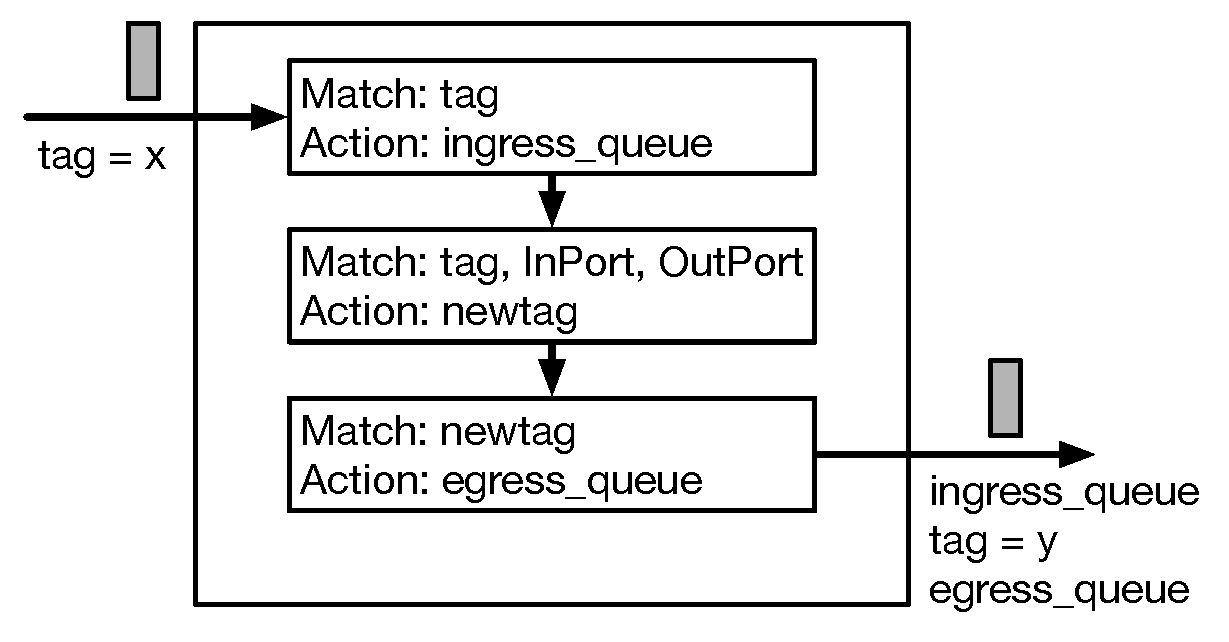
\includegraphics[width=0.42\textwidth] {figs/Tagger}
	%\vspace{-1em}
	\caption{Tagger match-action rules}\label{fig:tagger}
%	\vspace{-2em}
\end{figure}

\para {Match-Action rules:} \sysname{} needs to perform two operations at every
hop, i.e., {\em tag-based priority queueing} and {\em tag
rewriting}.  These two operations are implemented using a 3-step match-action
pipeline (Figure~\ref{fig:tagger}).  First, \sysname{} matches
the value of tags and classifies packets into ingress queues based. Second, 
\sysname{} matches (tag, InPort, OutPort) and rewrites the value of tag. 
The {\em third} step, wherein the packet is placed in an egress queue based on the
{\em new} tag value, is needed to ensure correct PFC operation, as described below.

\begin{figure}[t]
  %\vspace{-3em}
 	\centering
 	\subfloat[short for lof][Ingress priority = egress priority  $\rightarrow$ packet drop.] {
 	%	\vspace{-3em}
 		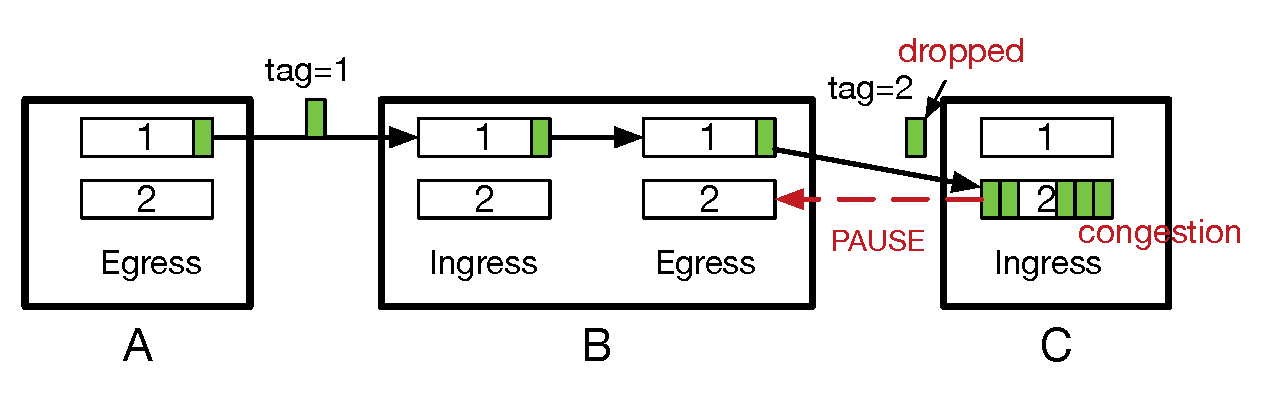
\includegraphics[width=0.42\textwidth] {figs/prioritydecoupling_1}
 	}
%  \vspace{-1.2em}
  
 	\subfloat[short for lof][Ingress priority = 1, egress priority = 2 $\rightarrow$ no drop.]{
 		%\vspace{-3em}
 		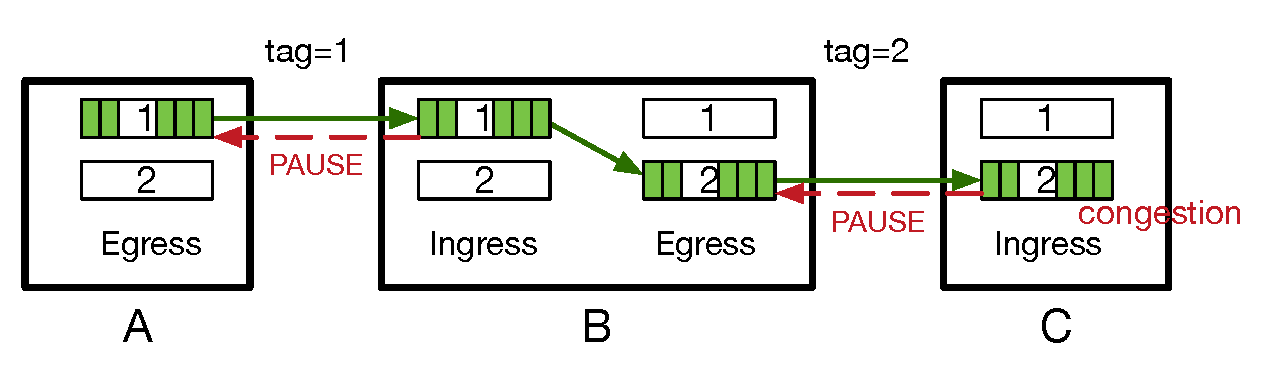
\includegraphics[width=0.42\textwidth] {figs/prioritydecoupling_2}
 	}
	 %\vspace{-1em}
 	\caption{Decoupling ingress priority from egress priority at switch B is necessary for lossless priority transition.}\label{fig:prioritydecoupling}
%	\vspace{-1em}
\end{figure}

\para{Handling priority transition:}
By default, a switch will enqueue a departing packet in the egress queue
of the same priority class as its ingress queue, as shown in Figure~\ref{fig:prioritydecoupling}(a).
In this example, Switch B is configured to 
perform priority transition for packets received from switch A and destined for switch C.
Packets exit egress queue 1 at switch B, but with priority 2. 
When ingress queue 2 of switch C becomes congested, the PFC PAUSE from switch C 
to switch B carries priority 2, and cannot pause the egress queue 1 of switch B.
This default behavior can lead to packet loss.

Therefore, we must map the packet to the egress queue
based on its new priority (Figure~\ref{fig:prioritydecoupling}(b)).  
This avoids packet loss, since the PFC from switch C
correctly pauses the queue on which the packet with the new tag would be
exiting.

\para{Rule compression:}  The match-action rules of \sysname{}
are implemented with TCAM. TCAM entries consist of {\em Pattern},
{\em Mask}, and {\em Result}. They refer to the pattern to be matched, the mask bits 
associated with the pattern and the action that occurs when a lookup hits the pattern, 
respectively.  One TCAM entry can have several Pattern-Mask pairs to match multiple packet header fields
simultaneously, e.g., an entry like (Pattern-1, Mask-1, Pattern-2, Mask-2, Result)
matches two fields simultaneously and fires only if both matches succeed.

\begin{figure}
	 
	\centering
	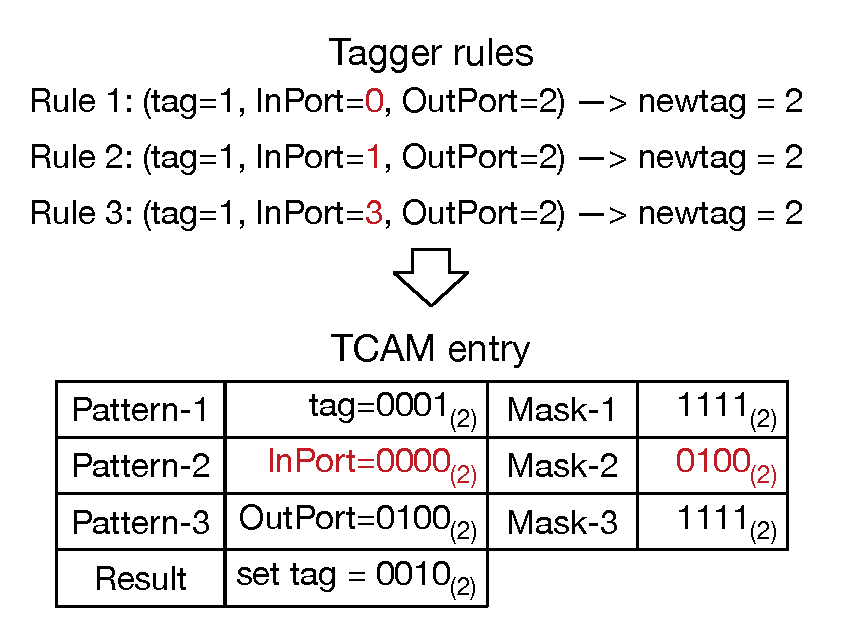
\includegraphics[width=0.37\textwidth] {figs/compression_with_bitmasking}
	\vspace{-1em}
	\caption{Rule compression with bit masking. Port numbers are bitmaps.
	The first bit from right represents port 0. The second bit represents port 1, and so on. }\label{fig:compression}
    \vspace{-1.5em}	
\end{figure}

Rules with the same Result can be compressed into one TCAM entry, if their
Patterns can be aggregated using bit masking. Consider the three
rules in Figure~\ref{fig:compression}. These rules are identical except the InPort
field in Pattern.

On commodity ASICs, port numbers in TCAM are bitmaps, not binary values. To match a single 
port, we can simply set the corresponding bit in the pattern to 1, and set the mask to all 1's. 
However, we may match multiple ports with one rule. We set the pattern to 
all 0's, and set the corresponding bits in the mask to 0. As shown in Figure~\ref{fig:compression},  
to match InPorts 0, 1 and 3, we set Pattern-2 to ``0000''  and Mask-2 to ``0100''. In this case, 
only the packet received from InPorts 0, 1 or 3 will match Pattern-2 after doing bit masking with Mask-2. 
Thus, the three rules are compressed into a single TCAM entry.

Recall from \S\ref{sec:generic} that without any compression, we need
$n(n-1)m(m-1)/2$ rules per switch. The number of rules can be
compressed to $nm(m-1)/2$ by aggregating InPorts.  The
result can be further improved by doing joint aggregation on tag, InPort and
OutPort.

\para{Broadcom implementation:} We implemented \sysname{} on commodity
switches based on Broadcom ASICs.  We use DSCP field in IP header as the tag.
The DSCP-based ingress priority queuing (step 1), ingress ACL and DSCP rewriting (step 2),
and ACL-based egress priority queuing (step 3) are well supported by the
commodity ASICs and do not require any ASIC changes. \shuihai{Everything is implemented using available and documented functionality.}

%Everything is implemented using publicly available and documented functionality.

%DSCP rewriting is supported by all commodity ASICs. DSCP-based priority
%queuing (step 1) is supported natively by all switch ASIC vendors. Step 2 uses
%ingress ACL rules to map (DSCP, InPort, OutPort) to new DSCP.

%Step 3 also uses ACLs, although it relies on certain details that are specific
%to Broadcom's match-action pipeline. We omit these gritty details for brevity.
%While the implementation of this step is Broadcom-specific, we believe that
%ASICs from other vendors can also support this functionality.

%%comment: this claim is not true, as brcm sdk is never public.
%%         
%We stress that none of the three steps require any changes to the switch ASIC,
%and everything is implemented using publicly available and documented
%functionality.

We considered using TTL instead of DSCP to tag packets, but TTL is automatically 
decremented by the forwarding pipeline, which complicates the rule structure.


	\section{Evaluation}\label{sec:eval}

We evaluate \sysname{} using a combination of testbed experiments and numerical
experiments. Our evaluation focuses on three key questions: $(i)$ Can \sysname{}
prevent deadlock? $(ii)$ Is \sysname{} scalable for large data center networks?,
and $(iii)$ Does \sysname{} have a performance penalty?

\begin{figure}
	\centering
	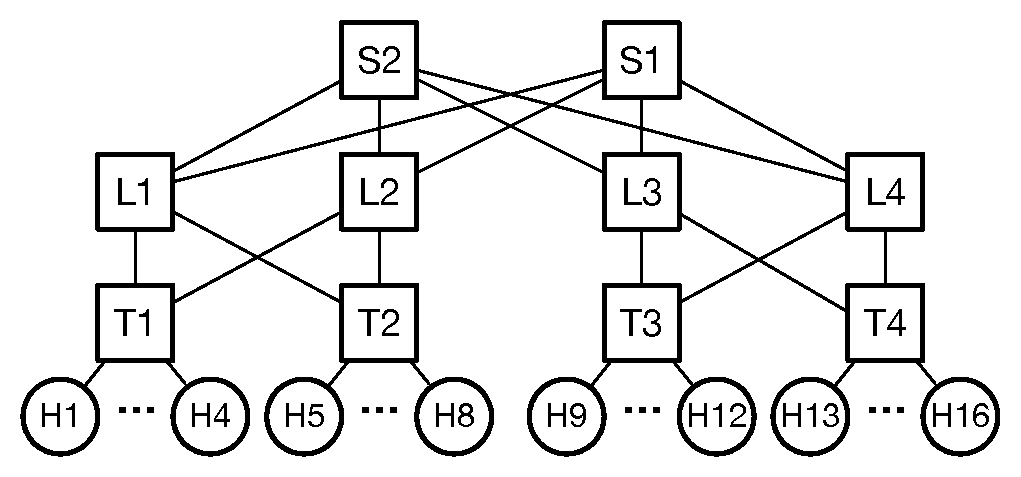
\includegraphics[width=0.45\textwidth] {figs/testbed_topo}
	\caption{Testbed Topology.}\label{fig:testbed_topo}
	\vspace{-0.25in}
\end{figure}

\para{Testbed:} Our testbed consists of a Clos network with 10 switches 16
servers (Figure~\ref{fig:testbed_topo}). Each server is a Dell PowerEdge R730
server with a 40GbE Mellanox ConnectX-3 Pro NIC. Each switch is a Arista
7050 switch with 32 40GbE ports and 16MB packet buffer. The switches
support PFC with at most 8 priority classes.




\subsection{Deadlock prevention}\label{subsec:exp_validation}

\begin{figure}[t]
	%\vspace{-0.1in}
	\centering
	
	\subfloat[short for lof][Without \sysname] {
		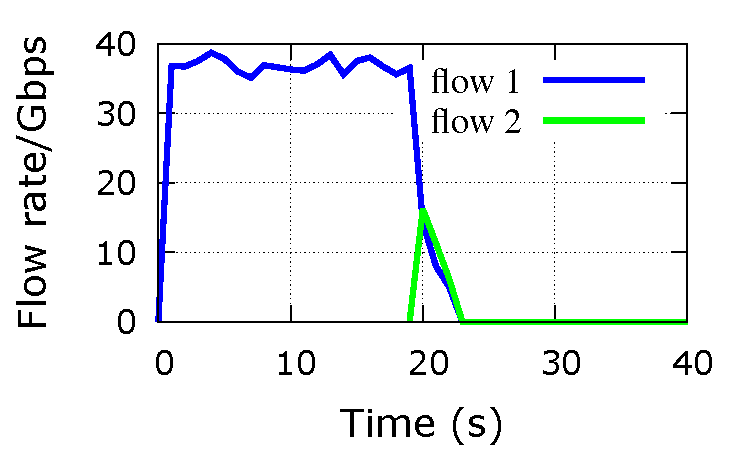
\includegraphics[width=0.25\textwidth] {figs/validation_nonloopcase_flowrate_notagger}
	}
	\subfloat[short for lof][With \sysname]{
		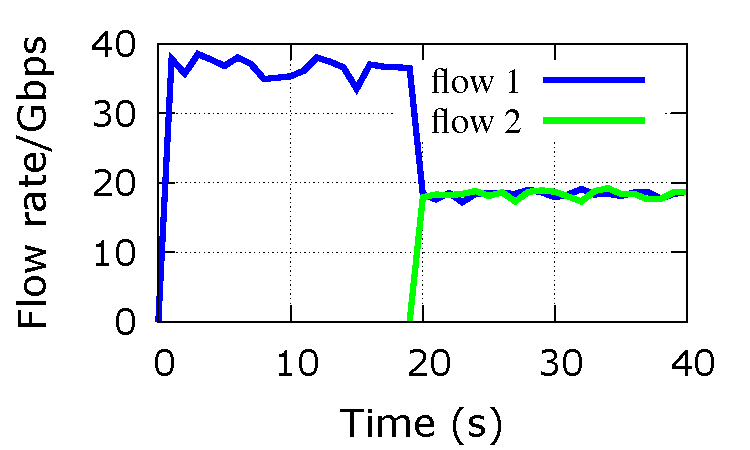
\includegraphics[width=0.25\textwidth] {figs/validation_nonloopcase_flowrate_tagger}
	}
	
	\caption{Clos deadlock due to 1-bounce paths}\label{fig:exp_validation_nonloop}
	\vspace{-0.25in}
\end{figure}

\begin{figure}[t]
	%\vspace{-0.1in}
	\centering
	
	\subfloat[short for lof][Scenario] {
		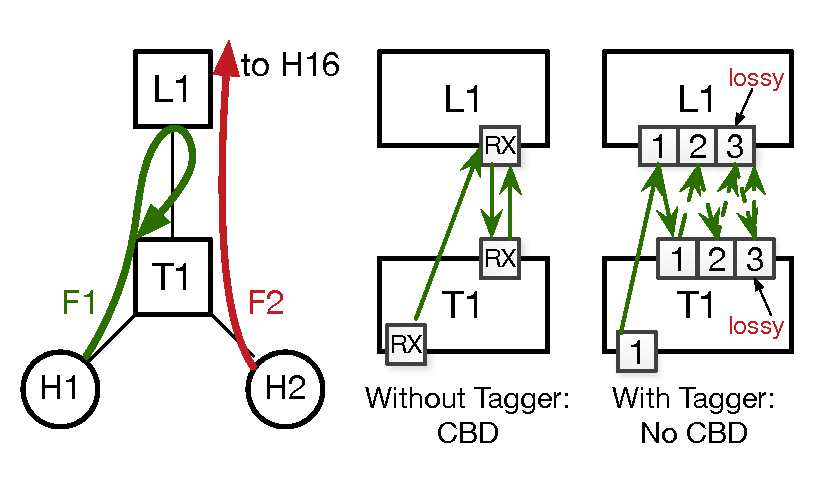
\includegraphics[width=0.4\textwidth] {figs/validation_loopcase_scenario}
	}

\vspace{-0.25in}

	\subfloat[short for lof][Rate of flow 2]{
		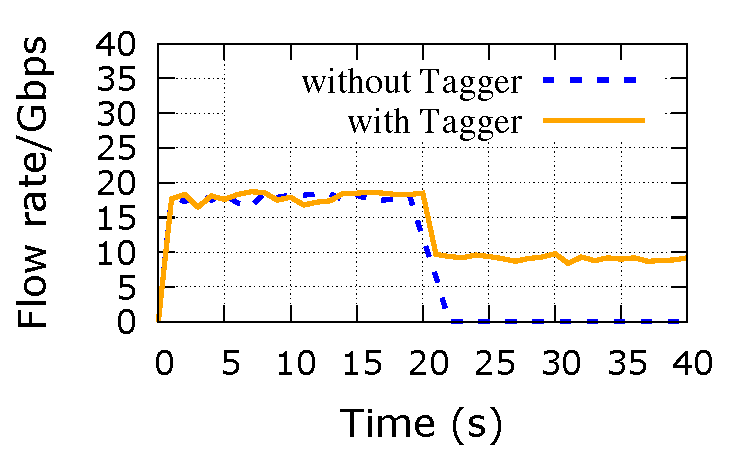
\includegraphics[width=0.4\textwidth] {figs/validation_loopcase_flowrate}
	}
	
	\caption{Deadlock due to routing loop}\label{fig:exp_validation_loop}
	
\end{figure}

\begin{figure}[t]
	%\vspace{-0.1in}
	\centering
	
	\subfloat[short for lof][4-to-1 shuffle with \sysname] {
		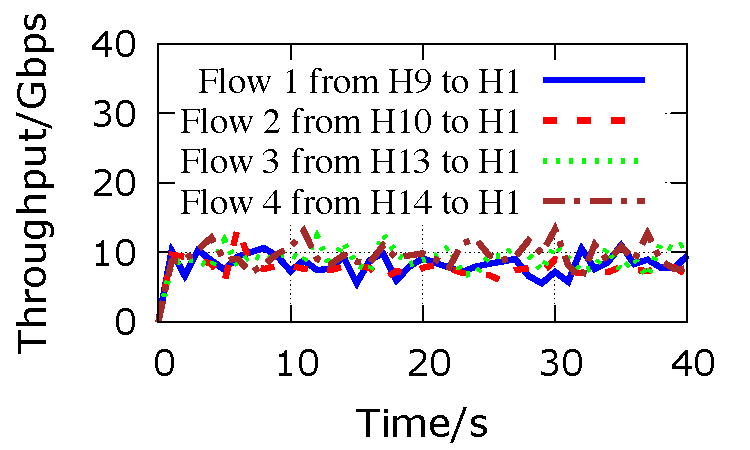
\includegraphics[width=0.25\textwidth] {figs/validation_pp_manytoone_tagger}
	}
	\subfloat[short for lof][4-to-1 shuffle without \sysname]{
		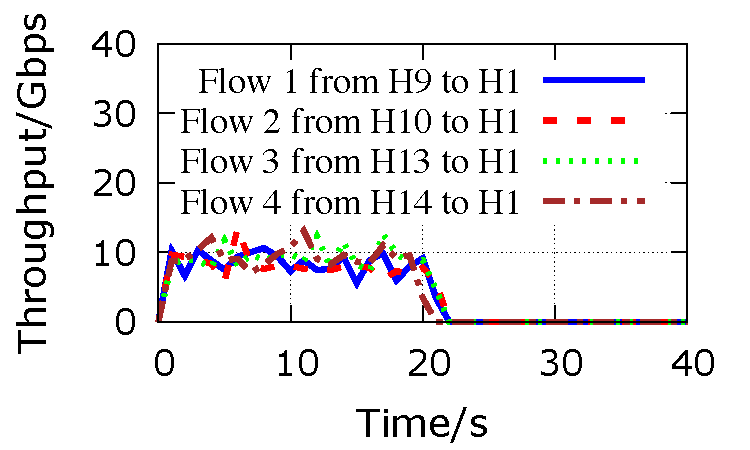
\includegraphics[width=0.25\textwidth] {figs/validation_pp_manytoone_notagger}
	}

	\subfloat[short for lof][1-to-4 shuffle with \sysname] {
	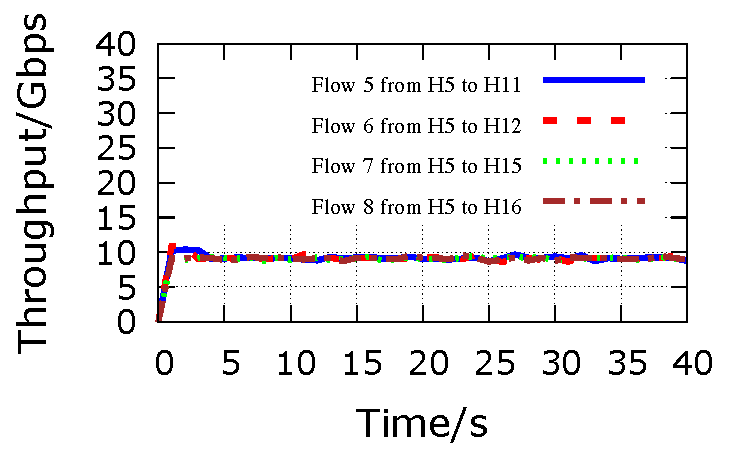
\includegraphics[width=0.25\textwidth] {figs/validation_pp_onetomany_tagger}
}
\subfloat[short for lof][1-to-4 shuffle without \sysname]{
	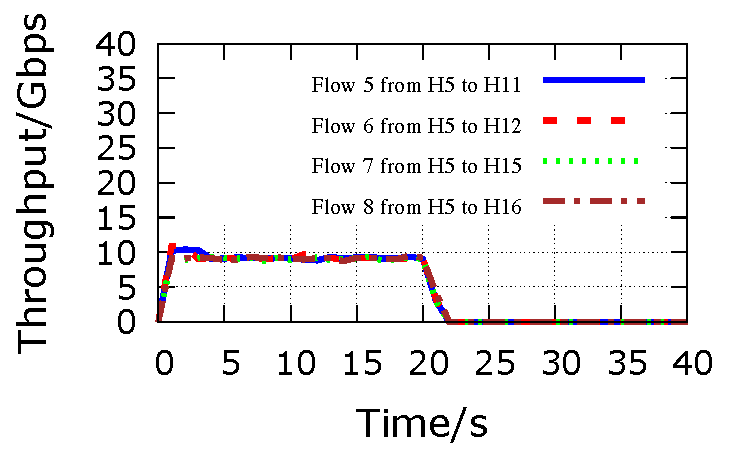
\includegraphics[width=0.25\textwidth] {figs/validation_pp_onetomany_notagger}
}
	
	\caption{PFC PAUSE propagation due to deadlock
	 }\label{fig:exp_validation_propagation}
	
\end{figure}


We have already {\em proved} that \sysname{} prevents deadlock, so the
experiments in this section are primarily illustrative. We have also done
extensive simulations. We omit these for lack of space.

\textbf{Deadlock due to one bounce:} We recreate the scenario shown in
Figure~\ref{fig:clos_1_bounce}, where 1-bounce paths lead to CBD.  In this
experiment, we start the orange flow at time 0, and the green flow at time 20.
Figure~\ref{fig:exp_validation_nonloop} shows the rate of the two flows with and
without \sysname{}.  Without \sysname{}, deadlock occurs and rate of both flows
are reduced to 0. With \sysname{}, and ELR set to include shortest paths and
1-bounce paths, there is no deadlock and flows are not paused.

\textbf{Deadlock due to routing loop:} As shown in
Figure~\ref{fig:exp_validation_loop}(a), we generate 2 flows across different
ToRs, i.e.,  $F_1$ from H1 to H15 and $F_2$ from H2 to H16. At time = 20s, we
install a bad route at L1 to let $F_1$ enter a routing loop between T1 and L1.
The path taken by $F_2$ also traverses link T1-L1.  ELR is set to include the
shortest paths and 1-bounce paths.

In Figure~\ref{fig:exp_validation_loop}(b), we plot the rate of $F_2$ with and
without \sysname{}. As we can see, if \sysname{} is not used, deadlock occurs
and $F_2$ is paused due to propagation of PFC PAUSE. With \sysname{}, there is
no deadlock and $F_2$ is not paused (but rate is affected by the routing loop). Note that
throughput of $F_1$ is zero, as packets are dropped due to TTL expiration.

The key takeaway here is that \sysname{} was able to successfully deal with a
routing loop.

\textbf{PAUSE propagation due to deadlock:} Once deadlock occurs, PFC PAUSE will
propagate and may finally pause all the flow running in the datacenter network.
In this experiment, we run a many-to-one data shuffle from H9, H10, H13 and H14
to H1, and a one-to-many data shuffle from H5 to  H11, H12, H15 and H16
simultaneously.  We then change the routing tables manually so that flow from H9
to H1 and the flow from H5 to H15 take 1-bounce paths. This creates CBD as
discussed earlier.

In Figure~\ref{fig:exp_validation_propagation}, we plot the throughput of all 8
flows with and without \sysname{}. Without \sysname{}, all flows get paused due
to PFC PAUSE propagation and throughput is reduced to zero. With \sysname{},
flows are not affected by link failures.

\subsection{Scalability}
\label{subsec:exp_overhead}

As discussed in \S\ref{sec:challenges}, commodity switches can support only a
limited number of lossless queues.  We have already shown that on a Clos
topology, \sysname{} requires $k+1$ lossless priorities to support paths with
up to $k$ bounces. We now consider other topologies.

\begin{table}[t]
		\footnotesize
	\centering
		\begin{tabular}{|r|r|r|r|r|}
			\hline
				Switches & Ports & Network & Lossless & Max \\
						 &		 & Diameter & Priorities & Rules \\
			\hline
			\hline
			100 & 32 & 6 & 3 &  37 \\
			\hline
			500 & 64 & 6 & 3 & 76 \\
			\hline
			1,000 & 64 & 6 & 3 & 88 \\
			\hline
			2,000 & 64 & 7 & 3 & 98 \\
			\hline
			2,000 (*)  & 64 & 7 & 4 &  135\\
			\hline
			
		\end{tabular} 
		\caption{Rules and priorities required for Jellyfish. Half the ports on
		each switch are connected to servers. ELP is shortest paths for first four entries. ELP for last entry includes additional 20,000 random paths.}
\label{table:jellyfish_shortestpath} \end{table}

Jellyfish topology is an r-regular random graph, characterized by the number of
switches, the number of ports a switch has (n) and the number of ports used to
connect with other switches (r).  In our experiment, we let r = n/2. Remaining
ports are connected to servers. We construct ELP by building destination-rooted
shortest-path spanning trees at all the servers.
Table~\ref{table:jellyfish_shortestpath} shows the results.  

\sysname{} requires only four classes for a network with 2000 switches, even
when 20,000 random routes are used in addition to the shortest paths, and at
most\footnote{Different switches require different number of rules due to the
random nature of the topology.} 135 match-action rules per switch.  Modern
commodity switches can support 1-4K rules, so this is not an issue. 

We also considered smaller (100 switches, 32 ports) Jellyfish topologies with
upto 16-shortest path routing. We need just 2 lossless priorities, and no more
than 47 rules per switch.

BCube~\cite{bcube} is server-centric topology, constructed from servers with $n$
ports, $n^k$ switches with $n$ ports. BCube$(8,3)$ with ELP of $3$ shortest
paths requires 4 lossless priorities, and 41 rules per switch.
F10~\cite{f10} is a fault-tolerant FatTree-like topology.  With three-level
network of 64 port switches, and ELP of all shortest and 1-bounce paths, we need
just 2 lossless priorities and 164 rules per switch.

Generating tagging rules is a one-time activity. Still, runtime of
Algorithm~\ref{alg:greedy} is of possible interest.
Figure.~\ref{fig:algo_runtime} shows the runtime for Jellyfish topologies of
different sizes. Even with 2000 switches, we complete rule generation in about
1.5 hours on a commodity desktop machine.

Thus, we conclude that in terms of number of lossless classes and ACLs,
\sysname{} scales well for modern data center architectures. 

\begin{figure}
	\centering
	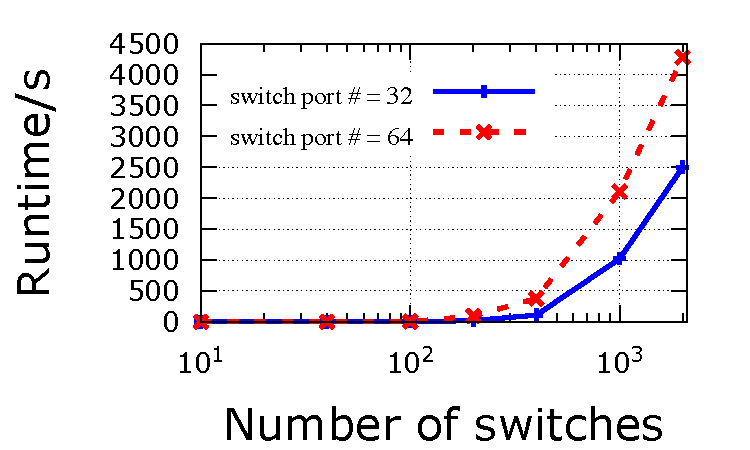
\includegraphics[width=0.45\textwidth] {figs/algo_runtime}
	\caption{Runtime of Algorithm~\ref{alg:greedy} for Jellyfish network of different sizes.}
	\label{fig:algo_runtime}
	\vspace{-0.25in}
\end{figure}

\subsection{Impact on throughout and latency}\label{subsec:exp_performanceoverhead}

\begin{figure}[t]
	\centering
	
	\subfloat[short for lof][Throughput] {
		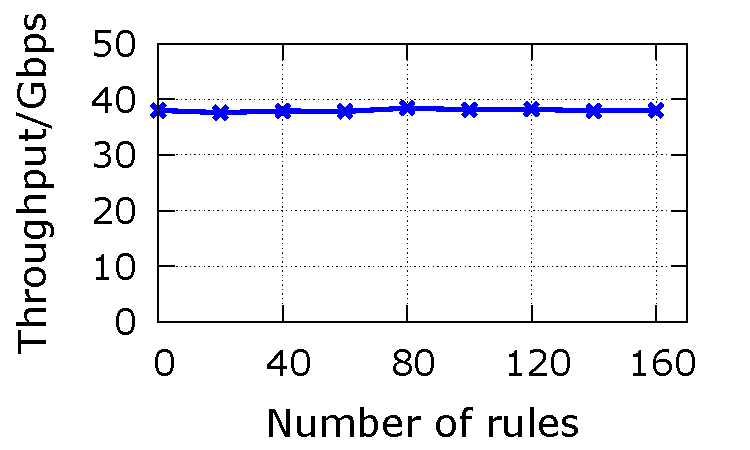
\includegraphics[width=0.25\textwidth] {figs/overhead_avgthrpt}
	}
	\subfloat[short for lof][Latency]{
		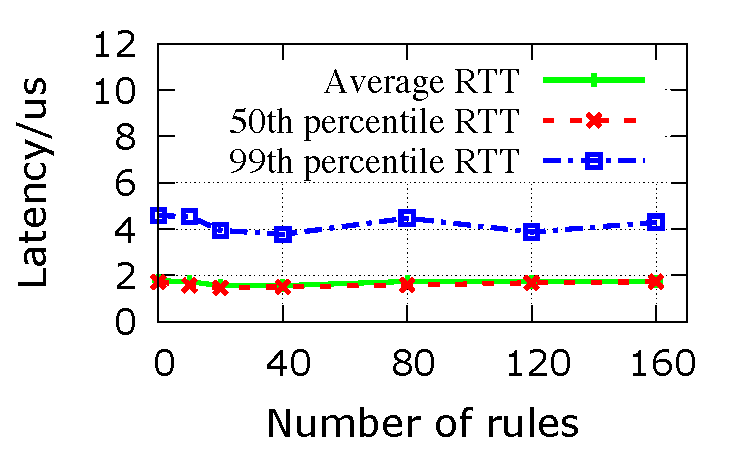
\includegraphics[width=0.25\textwidth] {figs/RDMAlatency_overhead}
	}
	
		\caption{\sysname{} has no impact on throughput and latency}
		\label{fig:perf_penalty}
	\vspace{-0.25in}
\end{figure}

At run time, the only impact of \sysname{} is that the packet has to traverse
the ACL rules. These are installed in TCAM, and hence have no discernible impact
on throughput and latency, as illustrated in Figure~\ref{fig:perf_penalty}.

\textbf{Throughput}: We generate one flow from H1 to H2, and observe its average
throughput over 100 seconds under varying number of \sysname{} rules installed
on T1. Figure~\ref{fig:perf_penalty}(a) shows that the average throughput is not
affected.

\textbf{Latency}: We install different number of \sysname{} rules in T1 and
collect 5000 RTT samples between H1 and H2.  Table~\ref{fig:perf_penalty}(b)
shows that latency is not affected.



%\subsection{Simple demonstration of \sysname{}}\label{subsec:exp_demon}  
%	
%	\begin{figure}[t]
%		%\vspace{-0.1in}
%		\centering
%		
%		\subfloat[short for lof][Experiment scenario.]{
%			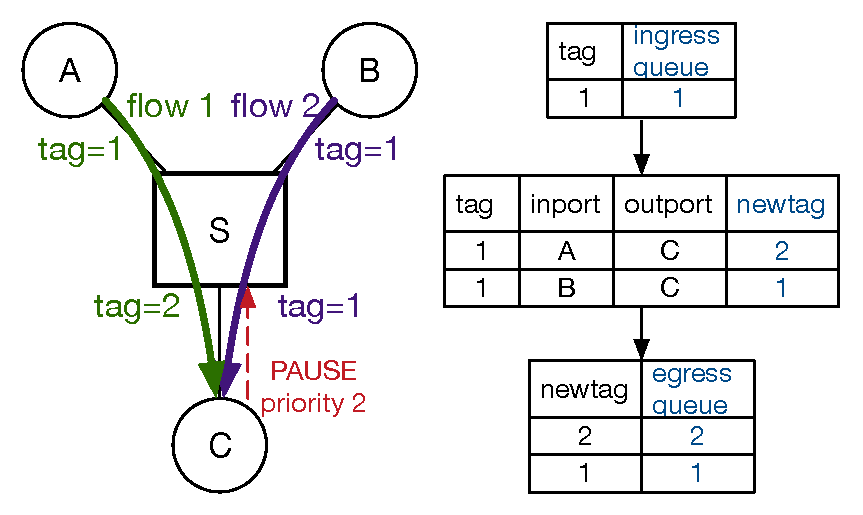
\includegraphics[width=0.25\textwidth] {figs/demon_scenario}
%		}
%		\subfloat[short for lof][Rate of flow 1 and flow 2.]{
%			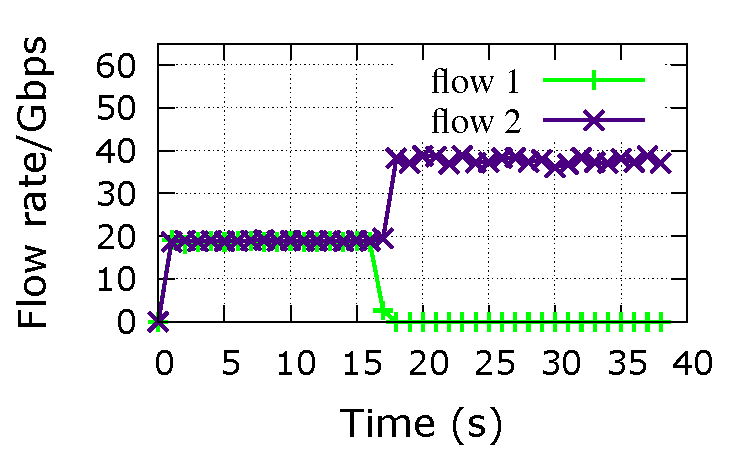
\includegraphics[width=0.25\textwidth] {figs/demon_flowrate}
%		}
%		
%		\caption{The match-action rules in action}\label{fig:tagger_demon}
%	\end{figure}
%	
%	
%A simple experiment shown in
%Figure~\ref{fig:tagger_demon} demonstrates the behavior of the match-action
%rules.  We generate two flows, flow 1 and flow 2, to send packets to C from
%different servers connected to ports A and B. Both servers set the DSCP value in
%outgoing packets to 1. The match-action rules are set to rewrite the tag value
%of packets arriving on port A to 2, and forward them to port C. Tag of packets
%arriving on port B is not changed.
%
%At time = 17s, C sends a stream of forged PFC PAUSE frames on priority 2 to
%switch S. The rate of both flows is plotted in Figure~\ref{fig:tagger_demon}(b)
%(link capacity = 40Gbps). As expected, after priority 2 is paused, rate of
%flow 1 is reduced to 0 while flow 2 gets all the available bandwidth.
%Counters on switch S further confirm that no packets were dropped, and server
%connected to port A was paused as expected.

	%\vspace{-0.1in}
\section{Related Work}\label{sec:related}

\para{Deadlock-free routing.} Many Deadlock-free routing designs have been
proposed. See
\cite{dally,duato93,dally93,sancho2004,flich2012survey,lash,wu2003fault,glass,duato2001,domke2011,puente1999,dfedst16}
for representative schemes. Generally, these designs prevent deadlock by
imposing restrictions on the routing paths, and can be classified into two
categories.

The first category is {\em deterministic routing based approach}, in which the
routing path is not affected by the traffic status, and there is no CBD.  These
routing algorithms are not compatible with existing routing protocols including
OSFP and BGP. Worse, they cannot be implemented in current commodity switching
ASICs.

TCP-Bolt~\cite{tcpbolt} and DF-EDST~\cite{dfedst16} are two recently
proposed deadlock-free routing designs. They both build edge-disjoint
spanning trees (EDSTs), with DF-EDST~\cite{dfedst16} further builds a
deadlock-free tree transition acyclic graph such that the transition
among some EDSTs can be allowed. However, existing L3 routing protocols
do not guarantee that packets will follow the pre-assign EDSTs, especially
upon link failures. Current switching ASIC cannot detect and handle all 
the potential EDST transition properly.

%support EDST.
%Furthermore, these designs need many EDSTs and
%every EDST needs to occupy a lossless queue. 
%Current switching ASIC,
%however, can only support 2-3 lossless queues.

The second category is {\em adaptive routing based approach.} The key idea is to
pre-install  ``escape'' paths at every switch to cover all possible
destinations. The switches can reroute packets to the ``escape'' paths in the
presence of congestion so that deadlock can be avoided.  As far as we know, no
commodity switching ASIC supports dynamic reroute based on traffic / queue
status.

\para{Intel Omni-Path.} Intel Omni-Path architecture \cite{omnipath} uses the
concept of Service Channels (SC) for routing deadlock avoidance.  Unlike
\sysname{}, Ommi-path uses a centralized fabric manager to manage the
network~\cite{omnipath}, including setting up SCs. This is not feasible at
data center scale.

%% Technical details of Omni-Path are not currently available, Tagger differs
%% from Omni-Path in two significant ways. First, Omni-path needs a fabric
%% manager to dynamically setup SC whereas the tag match-action rules are
%% pre-computed and statically configured. Second, Tagger enforces that
%% the tag of a packet increases monotonically whereas Omni-Path does not
%% enforce order for SC.

\para{Buffer management for deadlock prevention.} It has been shown that by
increasing the packet priority hop-by-hop, and putting packets of different
priority into different buffers, deadlock can be avoided
\cite{firstpaper,survey,datanetworks,karol2003prevention}. These designs,
however, need a large number lossless queues (which is the diameter of the
network). In \cite{dag}, the author tried to reduce the number of lossless
queues to only two. The design does not guarantee losslessness. Furthermore,
some switches need much larger buffer space than the others. 

\para{Deadlock recovery.} Deadlock recovery schemes
\cite{isca95,shpiner2016unlocking,venkatramani1996,martinez1997,Lopez1998}
detect deadlocks once they occur, and then try to break them by rerouting
packets.  These approaches have two issues: (1) They cannot guarantee that
deadlock will not happen again (if they can, there will be no need for deadlock
recovery). (2) They cannot be deployed using existing switch hardware.

%% need to add new deadlock detection algorithms and deadlock
%% breaking protocols into the switches.

%\para{Circuit switching-based approaches.} Those solutions from HPC and InfiniBand
%work by preemption. This does not work in Ethernet and in practice.

\para{Deadlock-free routing reconfiguration}:
Several deadlock-free routing reconfiguration schemes
\cite{automatic,lysne2005,doublescheme,gara2005} have been proposed for
ensuring deadlock-free during routing reconfiguration. \sysname{} can
be used to help any routing protocol to be deadlock-free, as
\sysname{} is decoupled from the routing protocols.

%The basic idea is to divide the reconfiguration process into multiple
%stages, and guarantee deadlock-free routing within each stage. We
%believe
%\sysname{} can be easily modified to guarantee deadlock-free of each
%reconfiguration stage.

\para{Summary.} \sysname{} is different from prior work because it works with
any routing protocol, and with existing hardware. We further have shown that
\sysname{} needs only small number of lossless queues.

%We believe that deciding the priority of packets along the path is
%better than changing routing configurations.

%Deadlock-free routing \cite{dally,duato93,dally93,sancho2004,flich2012survey,lash,wu2003fault,glass,duato2001,domke2011,puente1999} can be achieved by splitting the physical links into virtual channels and virtual channels are arranged in a way so as to avoid circular buffer dependency. In all those designs, the routing is decided by the virtual channels. Hence they cannot work with existing routing protocols for the data center networks which was designed for the lossy networks.
%can be achieved by splitting the physical links into virtual channels and virtual channels are arranged in a way so as to avoid circular buffer dependency. In all those designs, the routing is decided by the virtual channels. Hence they cannot work with existing routing protocols for the data center networks which was designed for the lossy networks.

%%TCP-Bolt~\cite{tcpbolt} uses multiple edge-disjoint spanning trees (EDSTs) and puts every EDST into a separate VLAN and lossless queue to achieve deadlock-free. In addition to the above drawbacks, to achieve good performance, TCP-Bolt may need a large number of lossless queues (which cannot be provided in current commodity switches). Furthermore, TCP-Bolt needs to run layer-2 VLAN, whereas all large-scale data center networks run layer-3.
%
%%DF-EDST~\cite{dfedst16} introduces a set of edge-disjoint spanning trees and a tree transition graph to provide deadlock free routing for arbitrary data center network topologies. DF-EDST, however, cannot work with existing routing protocols as it needs to follow the EDSTs. Furthermore, The EDST selection and transition cannot be readily implemented in current Ethernet switches.

	\secspacelarge
\section{Conclusion}
\secspace

In this paper, we studied the problem of deadlock in datacenter networks.  We
showed that CBD is a {\em necessary} by not {\em
sufficient} condition for deadlock formation. We are unable to fully characterize
the sufficient conditions, but using insights gained from a few examples, we
discussed potential deadlock mitigation mechanisms including TTL-based schemes,
rate limiting and reducing PFC propagation.


%	\begin{appendices}
\section{PFC headroom calculation}\label{APPHEADROOM}

The PFC headroom needed per port per lossless queue can be calculated by
		considering the time interval needed for a receiver to pause its
		upstream sender. The time interval is composed of the following 6
		periods for the lossless class $p$:

	
\noindent\textbf{The time to send a PAUSE frame $t_1$}.  Once a pause frame is
		generated, it may be blocked by a packet that has just started
		transmision. Since Ethernet is non-preemptive, in the worst-cast,
		$t_1 = \frac{ L_{mtu} + L_{pfc}}{B}$, where $L_{mtu}$ is the MTU size,
		and $L_{pfc}$ is the size of a PFC pause frame, and $B$ is the link
		rate.


\noindent\textbf{The PAUSE frame propagation time $t_2$}. This depends on 
		the cable length between the sender and receiver.

\noindent\textbf{The PAUSE frame receiving time at the sender $t3$}.
		$t_3=\frac{L_{pfc}}{B}$.

\noindent\textbf{The PFC response time $t_4$}. This is the amount of time needed
		for the sender to process the pause frame.

\noindent\textbf{The time for the sender to stop transmitting $t_5$}. Again,
		because Ethernet is non-preemptive, sender must to finish 
		transmitting the packet that may have already started. Hence, in the
		worst case, $t_5 =
		\frac{L^{p}_{mtu}}{B}$.

\noindent\textbf{The time for the pipe to be drained $t_6$}. We know $t_6 =
		t_2$.


At a first glance, the headroom size should be $B\times\sum t_i$. But there are
some additional details. The switching ASICs typically divide a packet
into small cells of equal size for internal packet storage and
processing. The cell size ($C$) is typically larger than the smallest
Ethernet packet size (64 bytes). For one 64-byte packet, one cell is
allocated. So in the worst-case, the needed headroom size is:
\begin{eqnarray} \label{eqn:pfcheadroom} S_{hdr} & = &
C\lceil\frac{(t_1+t_2+t_3+t_4 + t_6)B}{64}\rceil + C\lceil \frac{t_5
B}{64}\rceil \nonumber \end{eqnarray}

For a typical 40GbE RoCEv2 setup, we have $L_{mtu}=1500$ bytes, $L_{pfc}=64$
bytes, $t_2=t_6=1us$ (for about 200 meters cable length), $t_4=2.75us$,
$L^{p}_{mtu}=1100$ bytes, $C=208$ bytes.  For a commodity switch with 32
full duplex 40GbE ports, the total headroom size needed is 2.76MB for
supporting one lossless queue.  

\section{Optimal tagging scheme for Clos network}
\label{sec:clos_optimal}

Algorithm~\ref{alg:clos} produces optimal tagging for Clos networks. Note
similarity to Algorithm~\ref{alg:ttl}, except for the last step, which is
specific to Clos networks.

\begin{algorithm}
	\small
    \KwIn{Clos topology and lossless routes $R$}
	\KwOut{A tagged graph $G(V, E)$}
	$V \gets Set()$\;
	$E \gets Set()$\; 
	\For{each path $r$ in $R$} {
		$tag \gets 0$\;
		\For{each hop $h$ in $r$} {
			$V \gets V \cup \{(h, tag)\}$\;
			$E \gets E \cup \{lastHop\rightarrow(h, tag)\}$\;
			\If{$h$ is going down \&\& nextHop is going up} {
				$tag \gets tag+1$\;
			}
		}
	}
	\Return{$G(V, E)$}\;
    \caption{The optimal tagging system for Clos topology.}
	\label{alg:clos}
\end{algorithm}
\end{appendices}

	
	\bibliographystyle{acm}
	\bibliography{reference}
	
\end{document}
